\chapter{Beschreibung aus Anwendersicht} \label{anwendersicht}

Dieses Projekt ist für den Kunden entwickelt worden, daher wird hier die Anwendersicht beschrieben.

\section{Länderwahl}
\begin{figure}[h]
	\centerline{
		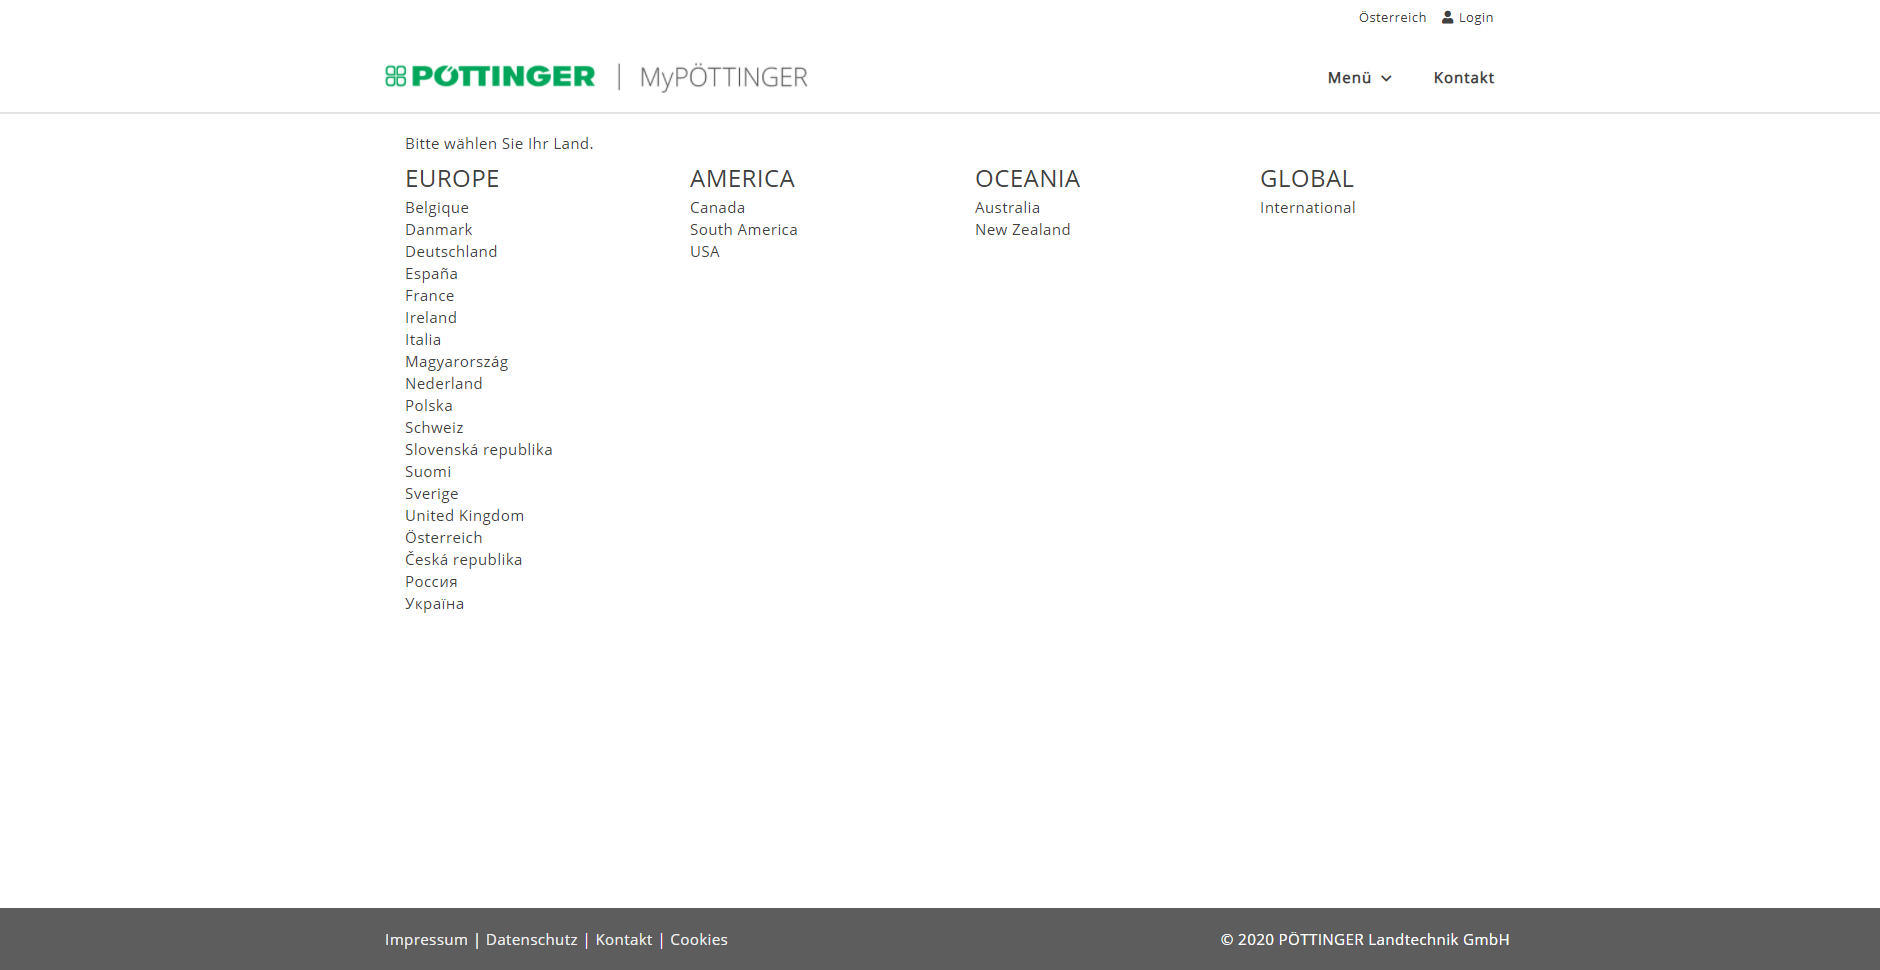
\includegraphics[width=1\textwidth, frame]{./grafiken/erm_country_selection.png}
	}
	\vskip0pt
	\caption{Screenshot von Länderwahl} \label{fig:countrySelection}
\end{figure}
Um auf die Webseite zu gelangen, ist es Erforderlicht, dass man davor in der Länderwahl, wie in Abbildung \ref{fig:countrySelection} sein Land und bei den Ländern, wo es mehrere Landssprachen gibt, auch die Sprache wählt. Aus dem Länder- und Sprachenkürzel setzt sich die Locale zusammen. Für Österreich wäre die Locale daher "de\_AT" und für Deutschland "de\_DE". Diese Locale wird in den Cookies gespeichert und die Webseite richtet sich nach dieser Locale in den Cookies. Es ist auch möglich, im Nachhinein das Land und die Sprache zu ändern, indem man im Header der Webseite auf das Land klickt. Durch diesen Klick gelangt man von überall auf die Länderwahl.

\section{Startseite}
\subsection{Startseite vor dem Login}
\begin{figure}[H]
	\centerline{
		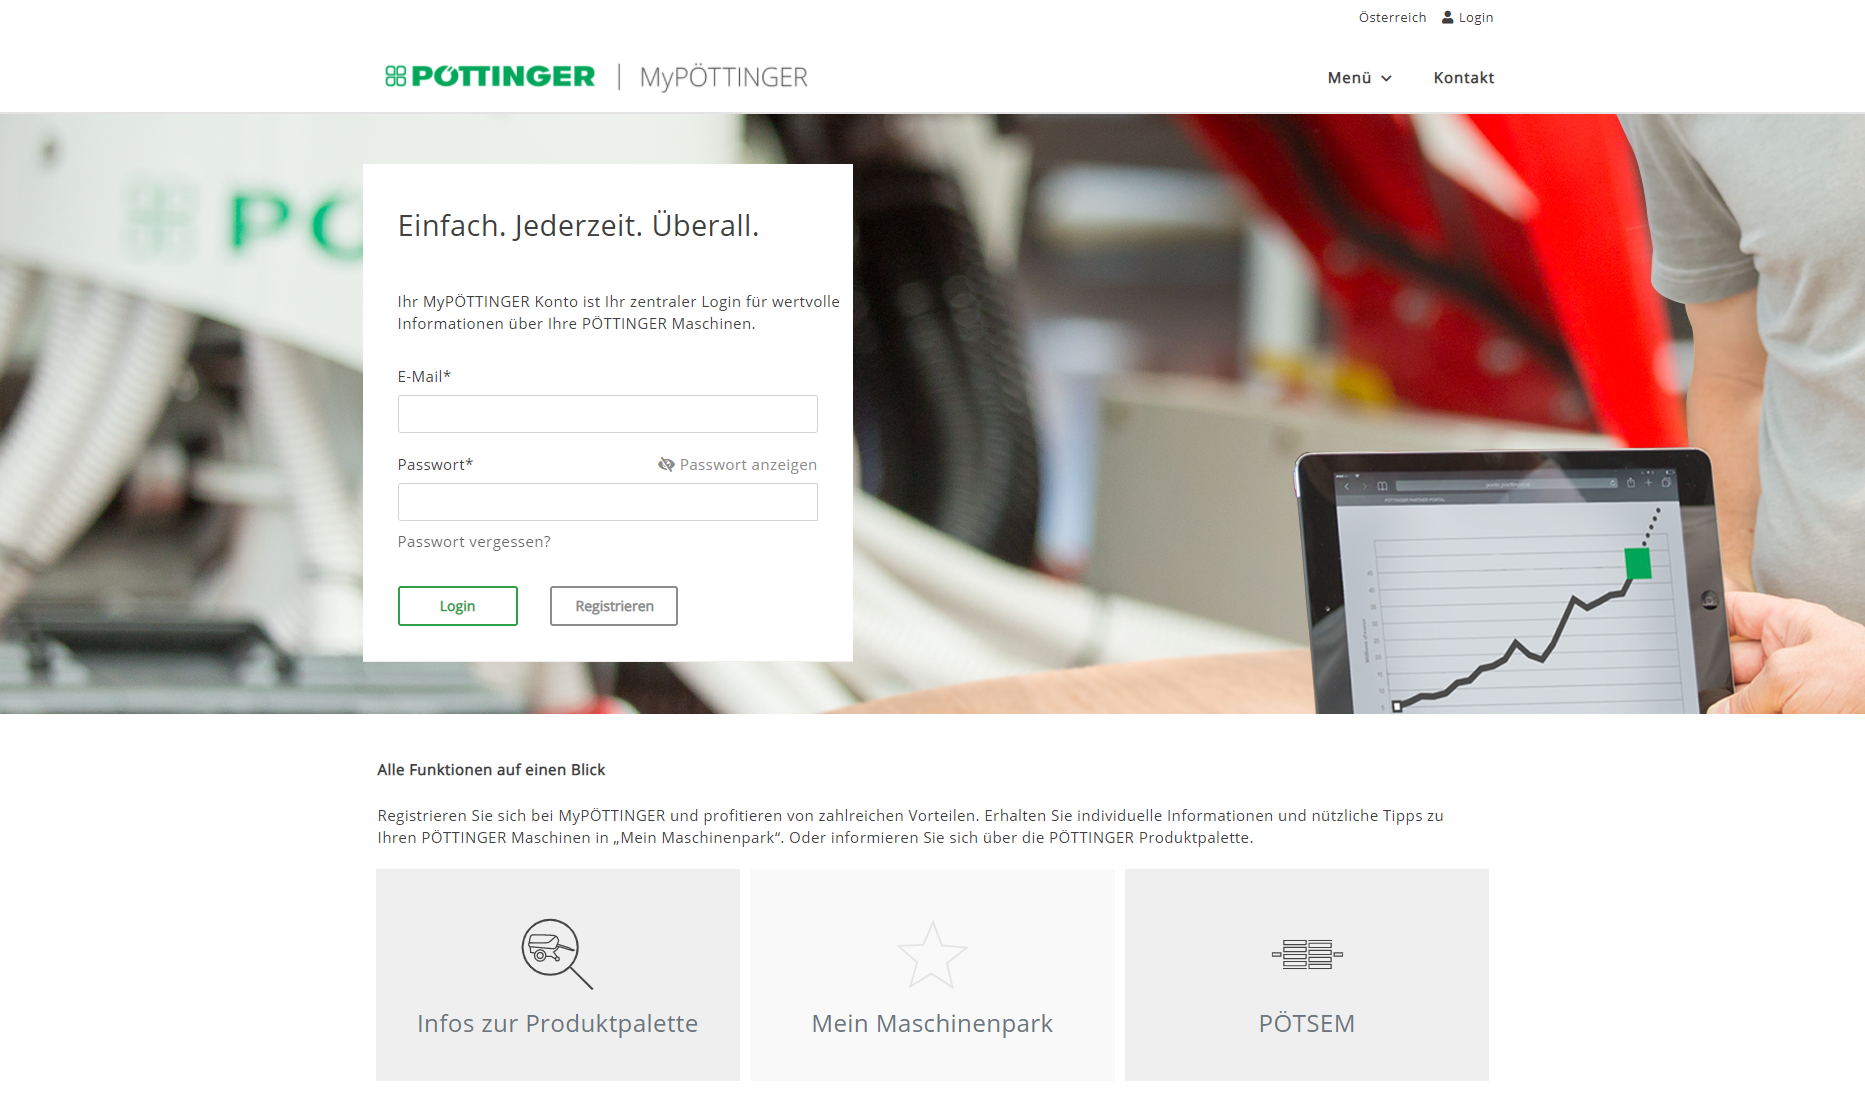
\includegraphics[width=1\textwidth, frame]{./grafiken/erm_home_not_logged_in_1.png}
	}
	\vskip0pt
	\caption{Screenshot von der Startseite nicht eingeloggt} \label{fig:homeNotLoggedIn}
\end{figure}

Nach der Länderwahl gelangt man zu der Startseite. Anfangs ist man noch nicht eingeloggt, daher ist ein Login-Feld in der Mitte, wie man in Abbildung \ref{fig:homeNotLoggedIn} sehen kann. Da sieht man auch, dass das Feld "Mein Maschinenpark" etwas heller ist als die anderen Felder, da man den Maschinenpark nur als eingeloggter Benutzer nutzen kann. Die zwei anderen Felder sind auch ohne Registrierung nutzbar.
 
\subsection{Startseite nach einem erfolgreichen Login}
\begin{figure}[H]
	\centerline{
		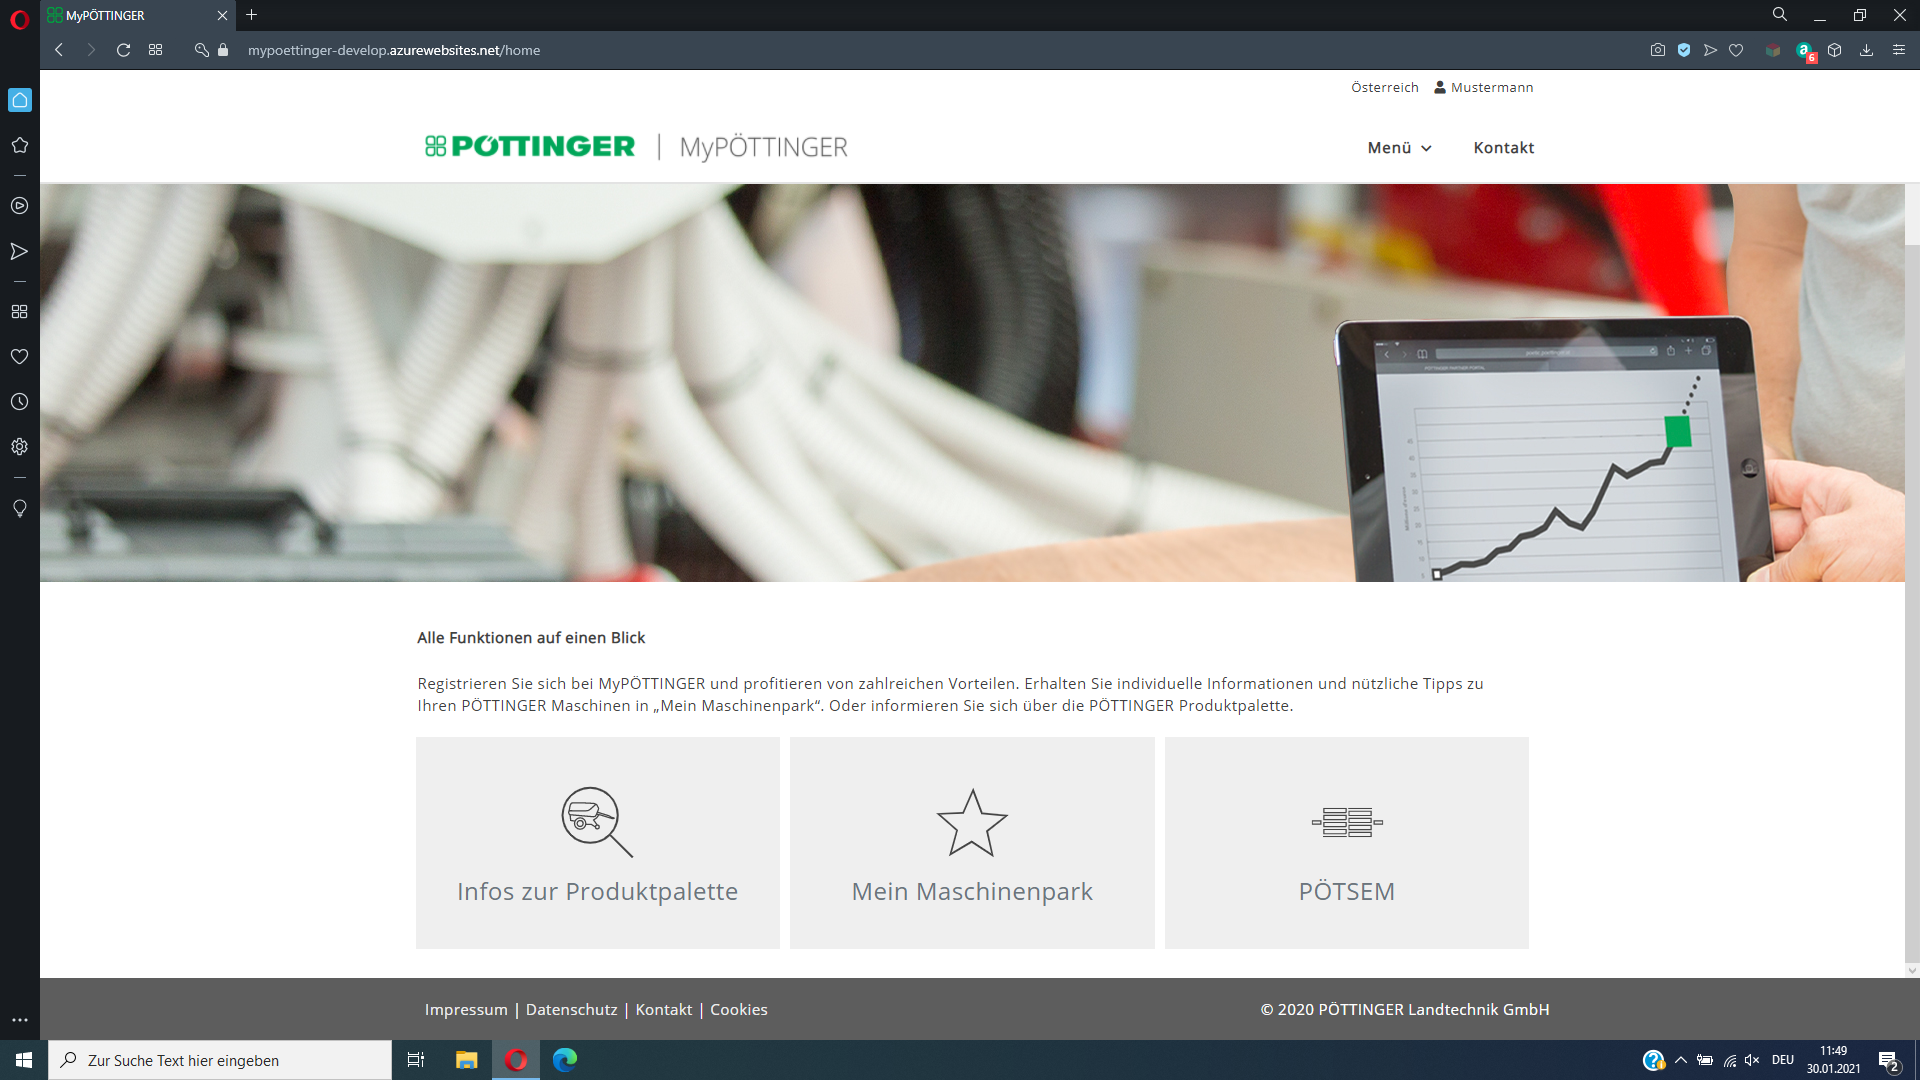
\includegraphics[width=1\textwidth, frame]{./grafiken/erm_home_logged_in.png}
	}
	\vskip0pt
	\caption{Screenshot von der Startseite eingeloggt} \label{fig:homeLoggedIn}
\end{figure}

Nach einem erfolgreichen Login ist das Feld "Mein Maschinenpark" aktiv. Als eingeloggter Benutzer hat man nun Zugriff auf den Maschinenpark. Das erkennt man, da das Feld in Abbildung \ref{fig:homeLoggedIn} den selben Grauton hat, als die beiden anderen Felder. 

\section{Registrierungsseite}

Falls man noch nicht registriert ist und man auf der Startseite auf "Registrieren" drückt, wird man zur Registrierungsseite weitergeleitet. Den ersten Teil dieser Seite sieht man in Abbildung \ref{fig:register}

\subsection{Registrierung}
\begin{figure}[H]
	\centerline{
		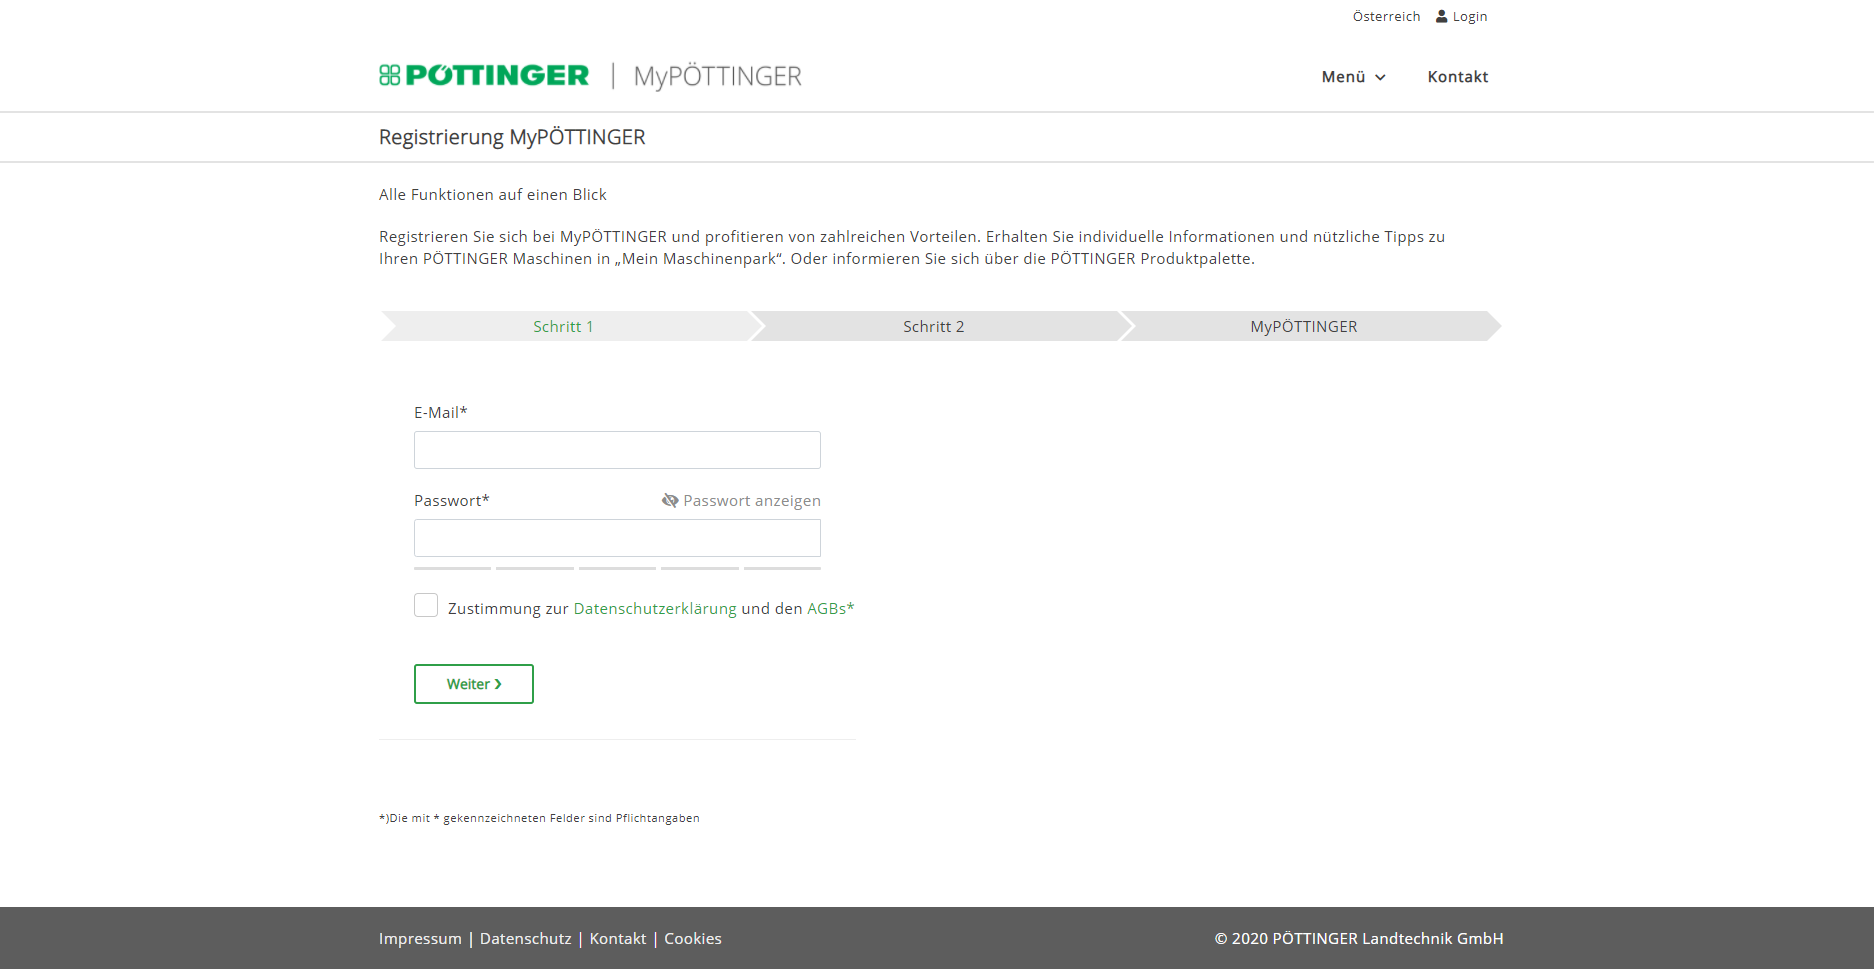
\includegraphics[width=1\textwidth, frame]{./grafiken/erm_register.png}
	}
	\vskip0pt
	\caption{Screenshot von der Registrierungsseite} \label{fig:register}
\end{figure}

Während der Passworteingabe bekommt man Feedback, wie sicher das ausgewählte Passwort ist und was noch fehlt, um den Passwortanforderungen zu entsprechen. Die Passwortanforderungen, die man in Abbildung \ref{fig:pwHints} sieht, entsprechen den Voraussetzungen von Auth0, da die Registrierung über Auth0 läuft. Der Balken unter dem Passwortfeld, wie in Abbildung \ref{fig:pwSec} gibt die Sicherheit des Passwortes an. Das Passwort wird mit gängigen Namen und Nachnamen aus Amerika, beliebte englische Wörter und Muster wie Datumsangaben, Wiederholungen und Tastaturmuster verglichen um die Stärke angeben zu können.

\begin{figure}[H]
	\centerline{
		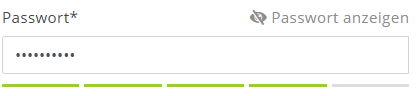
\includegraphics[width=1\textwidth, frame]{./grafiken/passwordSecurity.PNG}
	}
	\caption{Screenshot von der Passwortsicherheit} \label{fig:pwSec}
\end{figure}
\begin{figure}[H]
	\centerline{
	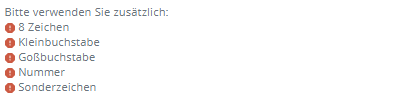
\includegraphics[width=1\textwidth, frame]{./grafiken/passwordHints.PNG}
	}	
	\caption{Screenshot von den Passworthinweisen} \label{fig:pwHints}
\end{figure}

\subsection{Weitere Daten für die Registrierung}

In diesem Schritt der Registrierung füllt man persönliche Daten aus. Das Land und die Sprache werden von der am Beginn ausgewählten Locale übernommen. Diese kann man aber auch hier noch ändern. Wenn das Land oder die Sprache geändert wird, wird dieses Formular neu generiert und die Felder werden nach den Standard des Landes erzeugt. Das bedeutet, dass die Reihenfolge der angezeigten Felder von dem ausgewählten Land abhängt, da in gewissen Ländern der Nachname vor dem Vornamen in einem Formular steht oder es in bestimmten Ländern Staaten oder Provinzen dazu kommen. Die Feldbeschreibung wird auch nach der ausgewählten Sprache geändert. Weiters wird auch die Validierung der Felder angepasst, denn zum Beispiel die Postleitzahl in den verschiedenen Länder variiert (4-stellig in Österreich, 5-stellig in Deutschland). \\
Für die Adresseingabe in der Abbildung \ref{fig:register2} hat der Benutzer 3 Möglichkeiten:\\
Es besteht die Möglichkeit, jedes Adressfeld selber auszufüllen. Somit sind die Felder Straße und Hausnummer, Ort, Postleitzahl und bei gewissen Ländern die Provinzen oder Staaten auszufüllen.\\
Eine etwas schnellere Variante ist die Verwendung von dem integrierten Typeaheads. Bei der Eingabe des Feldes Straße und Hausnummer erscheinen Adresseingabevorschläge darunter. Wenn man auf die gewünschte Adresse klickt, werden die Felder Ort, Postleitzahl und falls vorhanden die Provinz oder der Staat automatisch ausgefüllt. Alle Vorschläge, die angezeigt werden, sind in den ausgewählten Land. Somit wird verhindert, dass der Benutzer eine Adresse eingibt, die sich nicht in dem gewählten Land befindet.\\
Die schnellste Variante ist die Verwendung von der integrierten Standorterkennung. Dafür drückt man den "Use my location" über dem Adressfeld. Dadurch wird der Standort bestmöglich erkannt und alle vorhandenen Adressfelder werden automatisch ausgefüllt. Falls der Standort nicht ganz richtig erkannt wurde, kann man es danach noch bearbeiten. Die Standorterkennung ändert auch das ausgewählte Land, falls diese nicht übereinstimmen.
\begin{figure}[H]
	\centerline{
		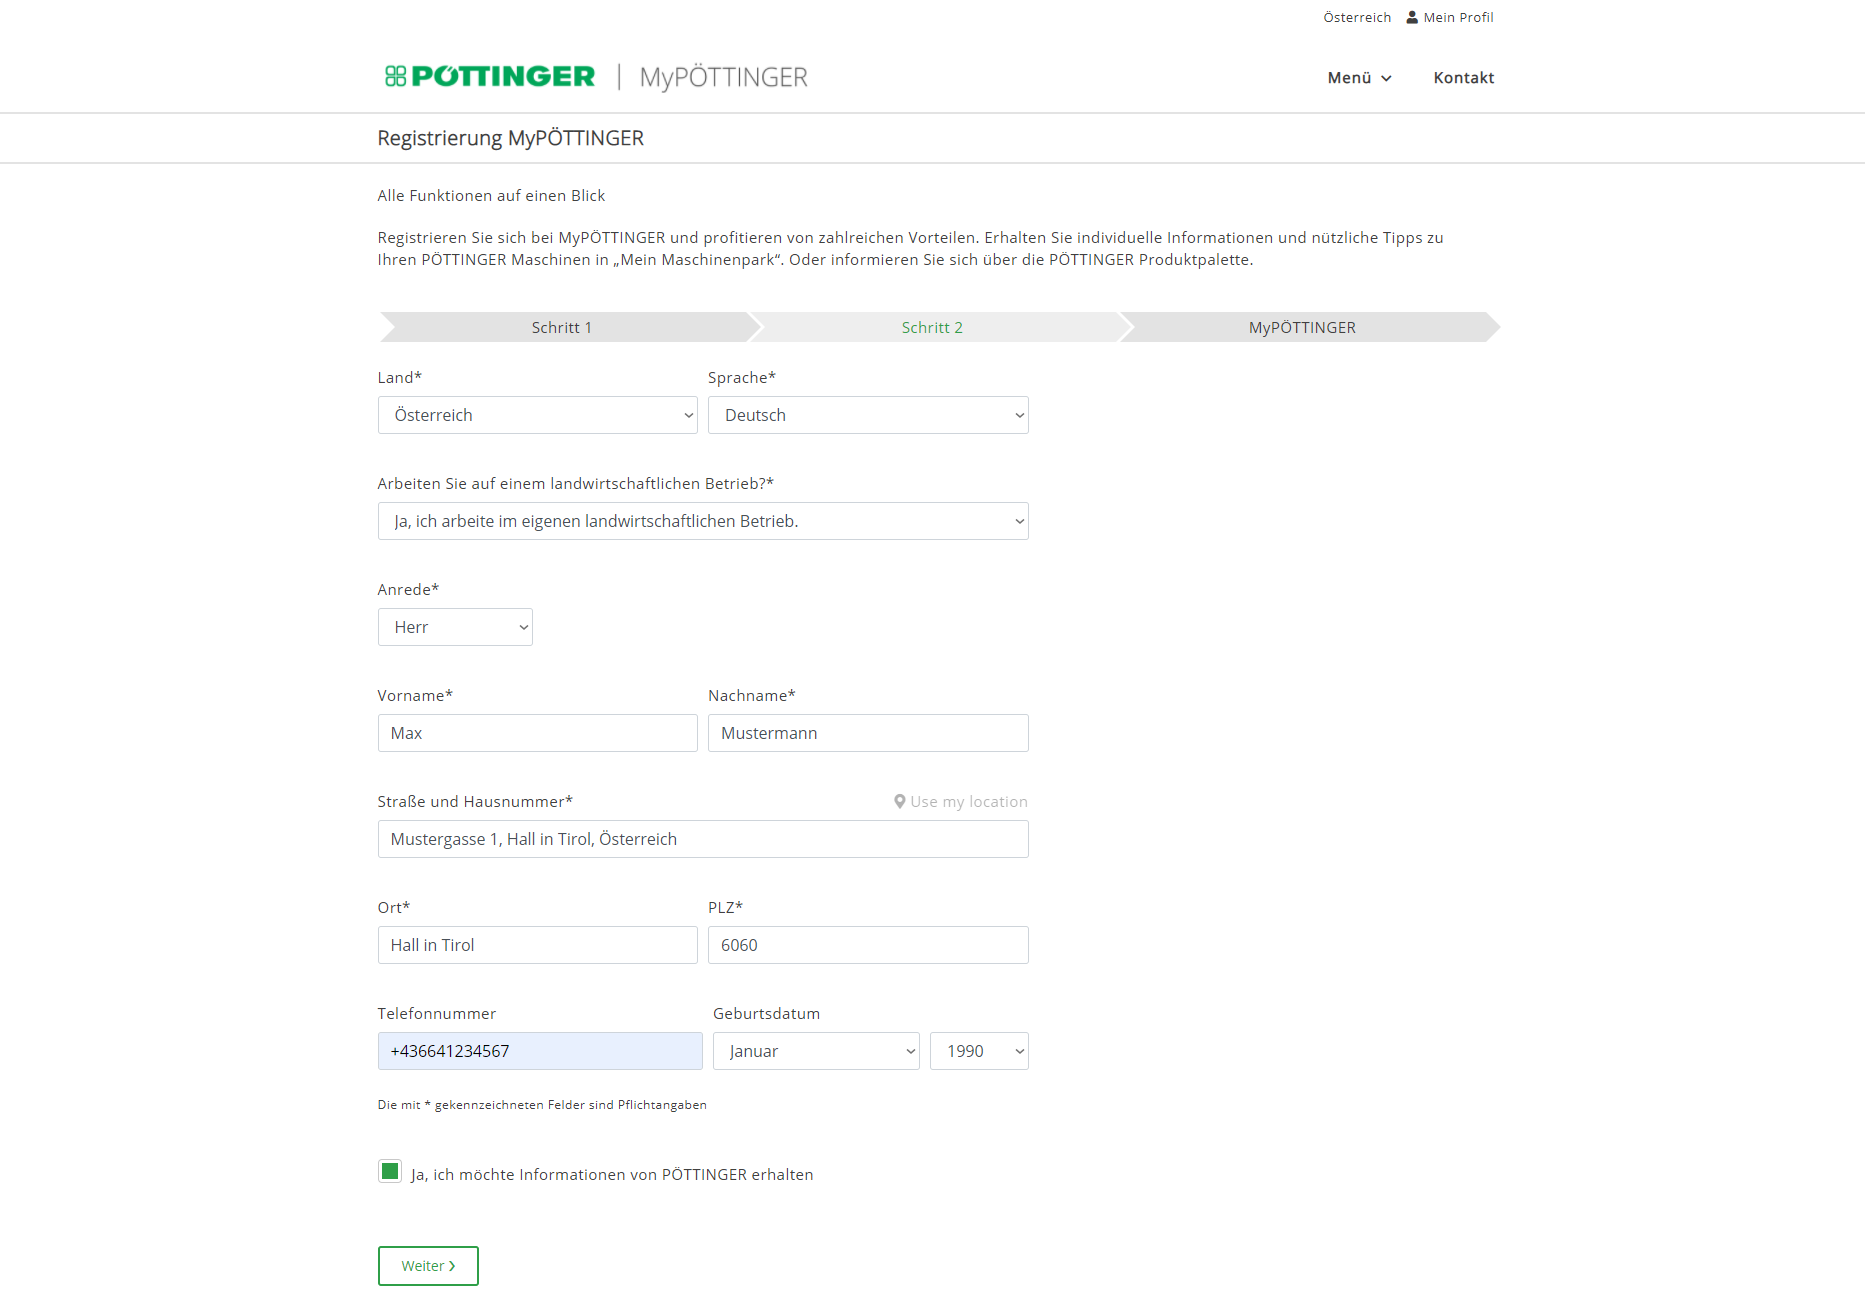
\includegraphics[width=1\textwidth, frame]{./grafiken/erm_register_data.png}
	}
	\vskip0pt
	\caption{Screenshot von der Dateneingabe der Registrierung} \label{fig:register2}
\end{figure}

Um anzugeben, ob der Benutzer auf einem landwirtschaftlichen Betreib arbeitet, besteht die Möglichkeit, dass er auf dem eigenen landwirtschaftlichen Betrieb arbeitet, auf einem anderen landwirtschaftlichen Betrieb angestellt ist oder dass er auf keinen Betrieb arbeitet. Falls der Benutzer auswählt, dass er auf einen anderen Betrieb angestellt ist, erscheint zusätzlich das Feld für den Namen des Unternehmens.\\
Jedes Eingabefeld wird sofort nach Abgabe des Cursorfokus validiert. Falls ein Fehler auftritt wird das Feld rot umrandet und unter dem Feld erscheint eine Fehlermeldung, was falsch ist. Die Eingaben werden im Frontend und im Backend validiert. In der Abbildung \ref{fig:eingabeError} sieht man die Felder mit einigen möglichen Fehlermeldungen. Bei einer korrekten Eingabe, verschwindet der rote Rahmen um das jeweilige Feld wieder.
\begin{figure}[H]
	\centerline{
		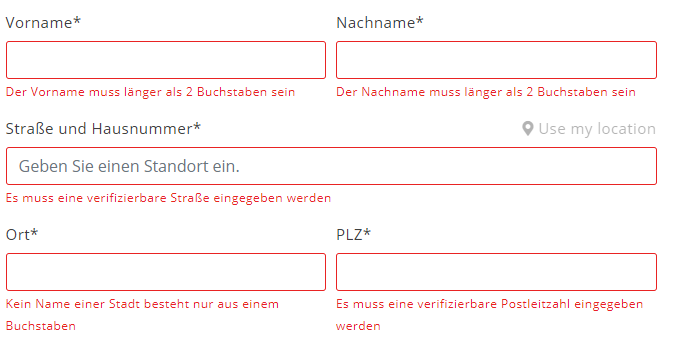
\includegraphics[width=1\textwidth, frame]{./grafiken/dateneingabe_Errors.PNG}
	}
	\vskip0pt
	\caption{Screenshot von den Fehlermeldungen der Eingaben} \label{fig:eingabeError}
\end{figure}

\subsection{Letzter Schritt der Registrierung}
Um die Registrierung erfolgreich abzuschließen, bekommt man eine Bestätigung per E-Mail zugesendet. Darin befindet sich ein Aktivierungslink. Den letzte Schritt der Registrierung sieht man in der Abbildung \ref{fig:step3register}. Hier wird man nur mehr gebeten, den Link in der E-Mail zu klicken. Nach der Aktivierung ist die Webseite ohne Einschränkungen nutzbar.
\begin{figure}[H]
	\centerline{
		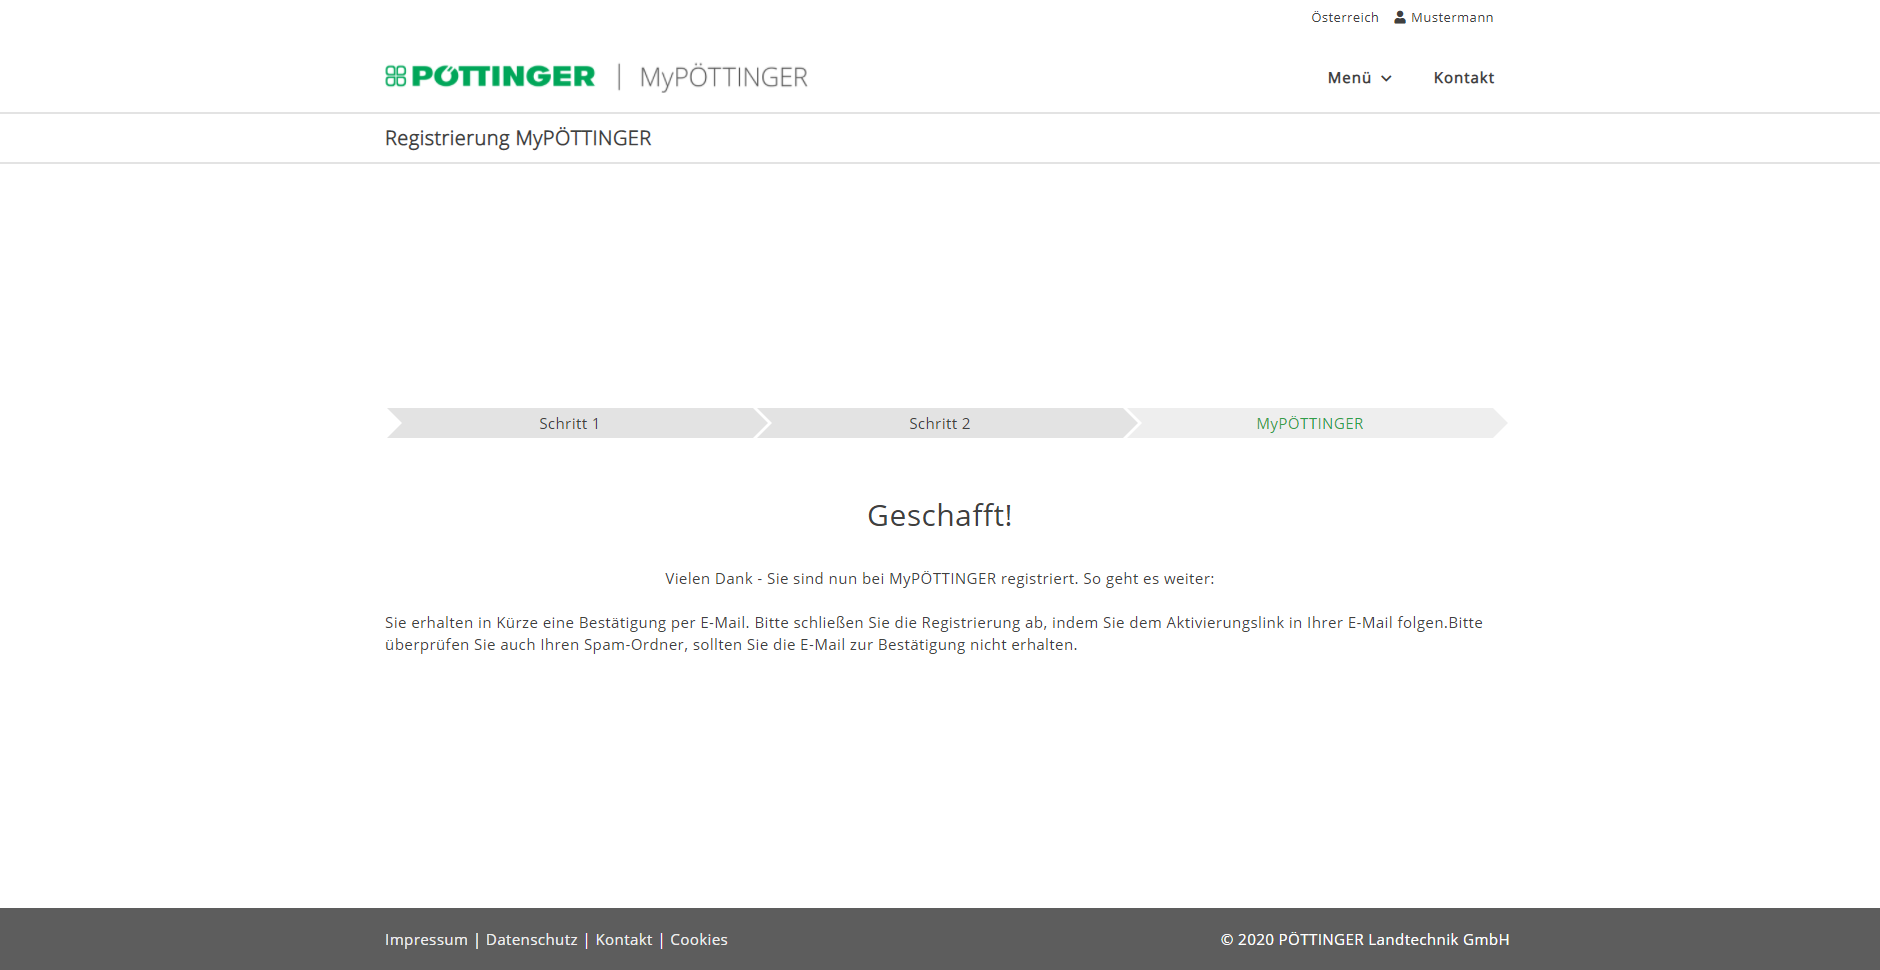
\includegraphics[width=1\textwidth, frame]{./grafiken/erm_register_final.png}
	}
	\vskip0pt
	\caption{Screenshot von dem letzten Schritt der Registrierung} \label{fig:step3register}
\end{figure}

Nach der Bestätigung in der E-Mail wird man zurück auf die Startseite geleitet und es erscheint ein Pop-Up, wie man in Abbildung \ref{fig:popup} sieht.

\begin{figure}[H]
	\centerline{
		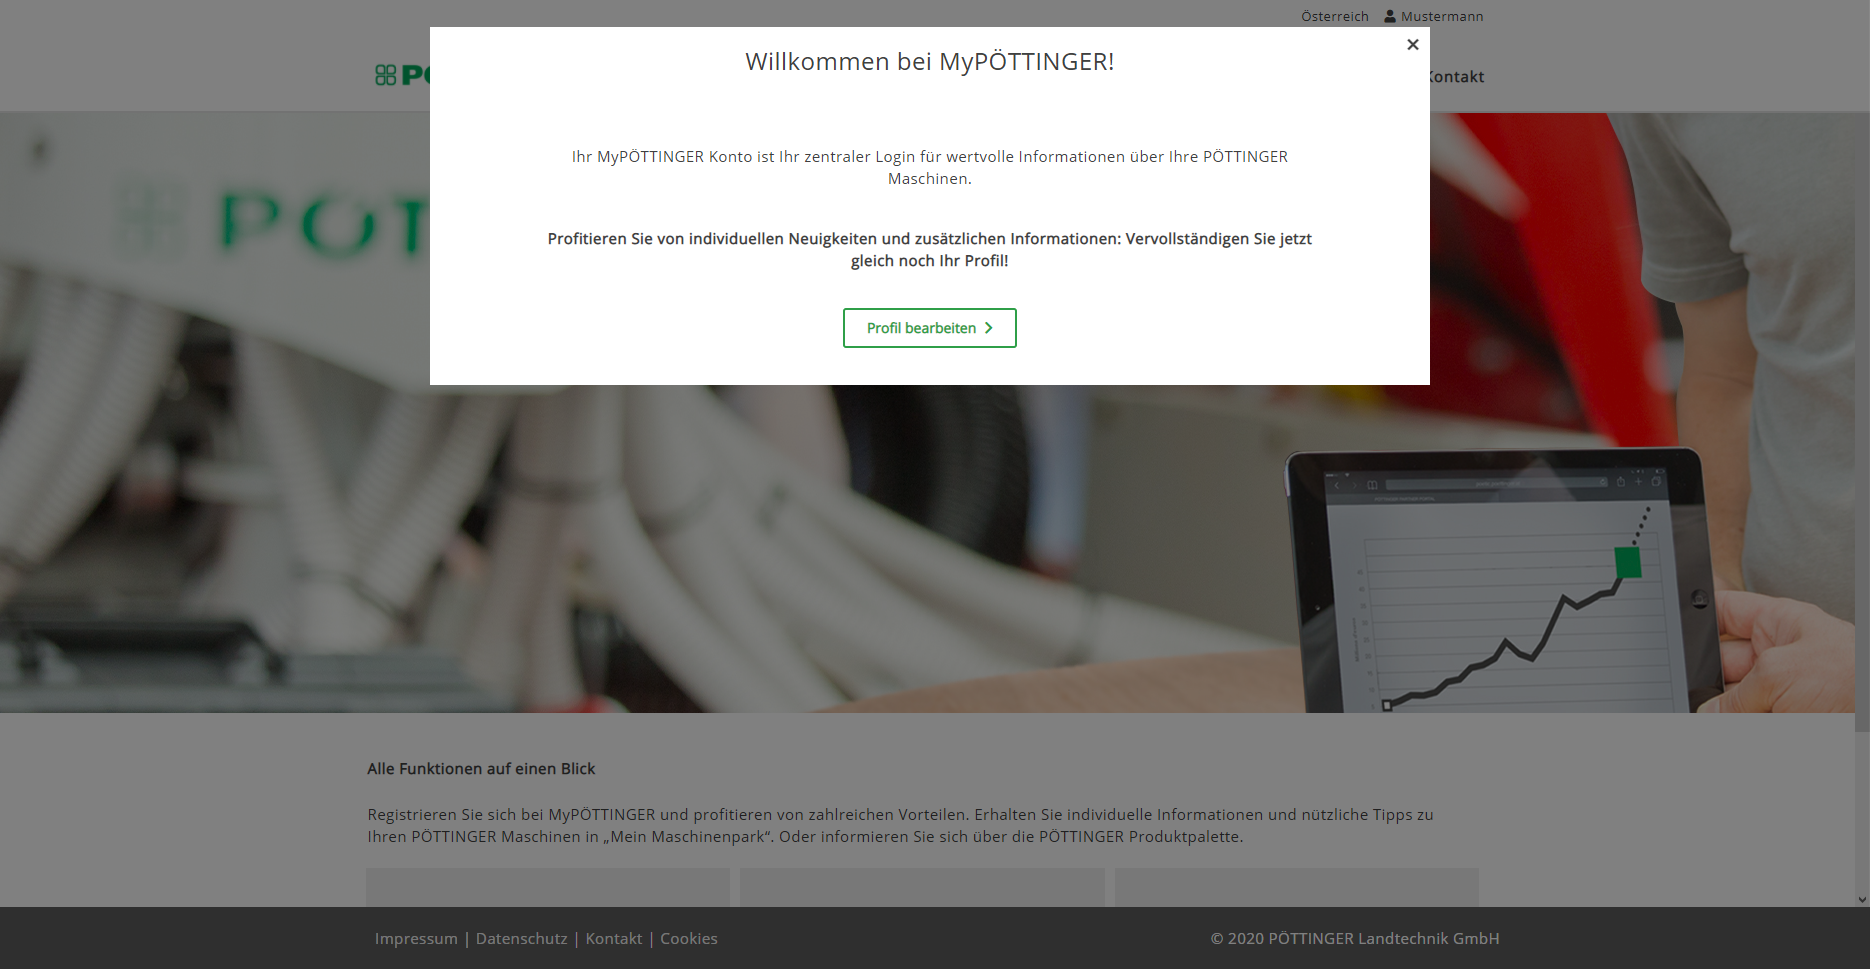
\includegraphics[width=1\textwidth, frame]{./grafiken/erm_home_after_email.png}
	}
	\vskip0pt
	\caption{Screenshot von dem Bestätigungs-Pop-Up} \label{fig:popup}
\end{figure}

\section{Profilübersicht}

Auf die Profilübersicht gelangt man, wenn man in dem Bestätigungs-Pop-Up auf "Profil bearbeiten" klickt oder man klickt auf den eigenen Namen rechts oben und danach auf "Mein Profil". Die Profilübersicht sieht man in Abbildung \ref{fig:profil}.

\begin{figure}[H]
	\centerline{
		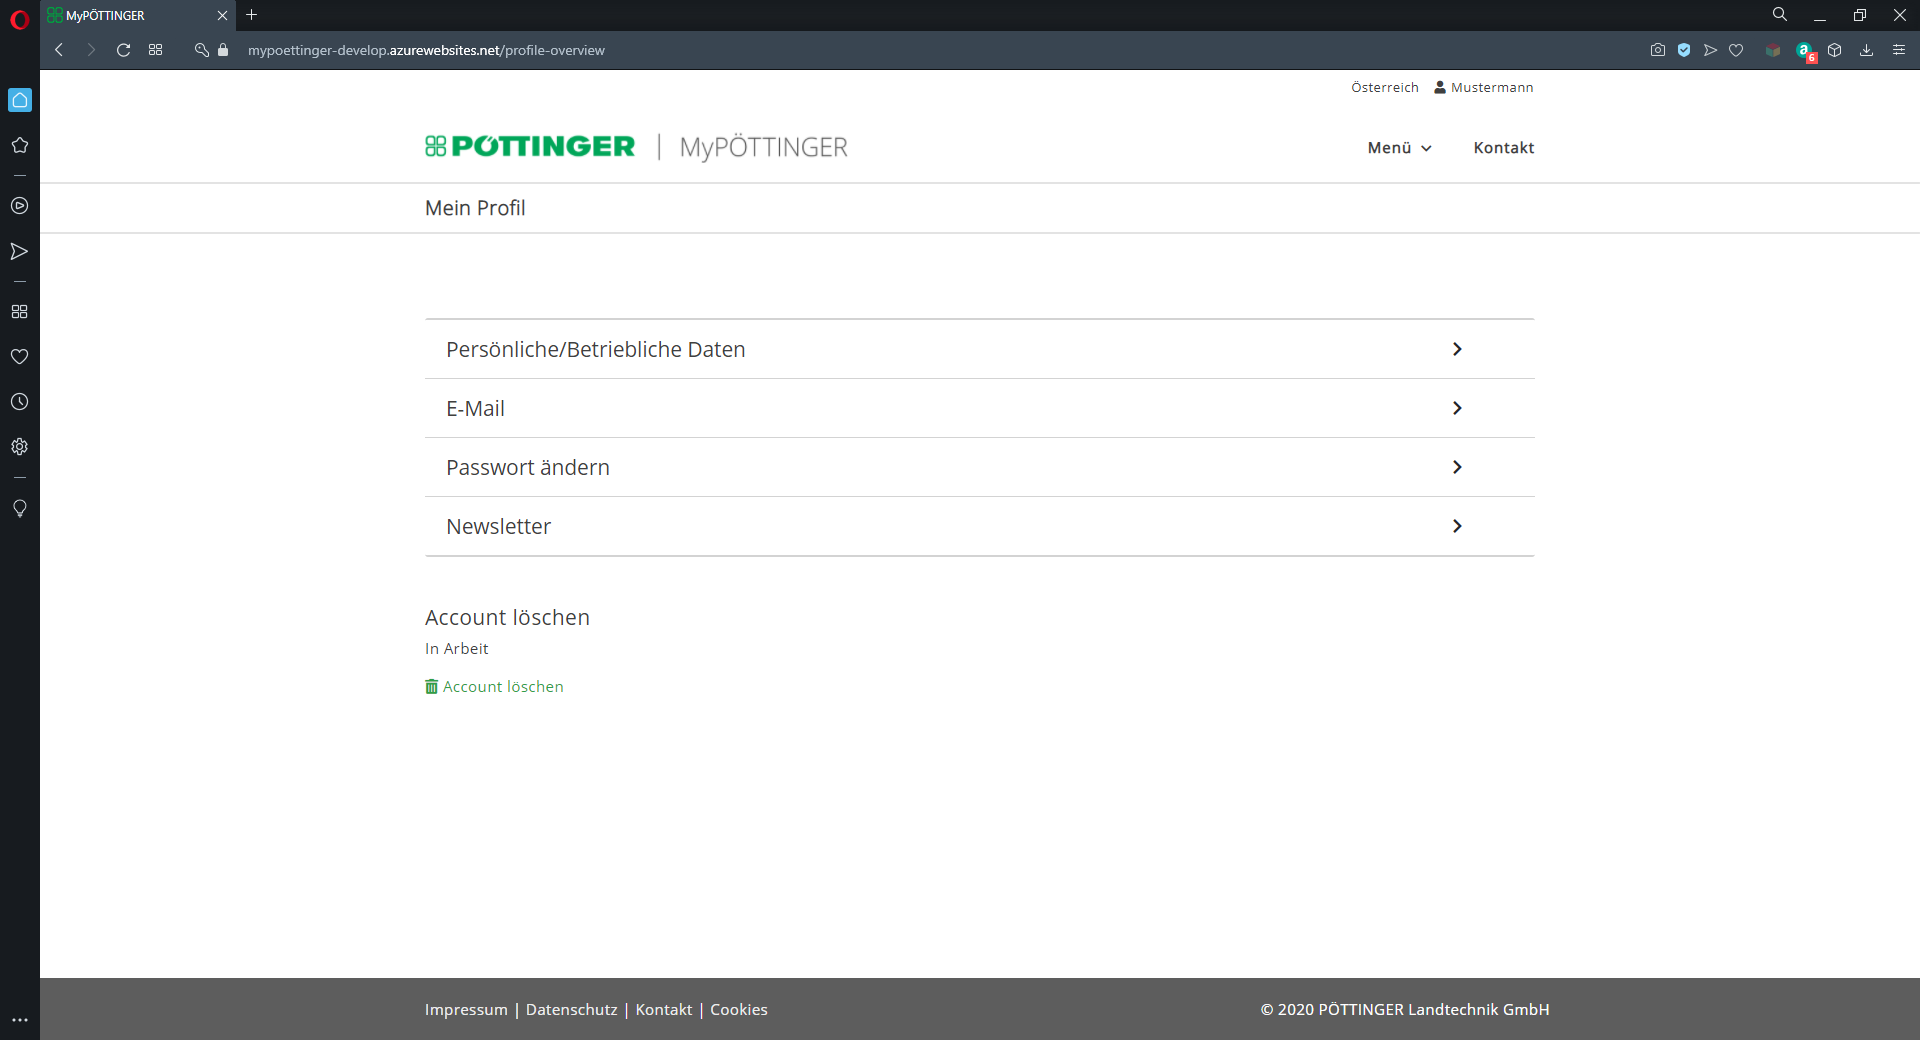
\includegraphics[width=1\textwidth, frame]{./grafiken/erm_profil.png}
	}
	\vskip0pt
	\caption{Screenshot von der Profilübersicht} \label{fig:profil}
\end{figure}

In der Profilübersicht kann man all seine persönlichen Daten einsehen und diese auch bearbeiten. Es besteht auch die Möglichkeit, die E-Mail und das Passwort zu ändern.

\subsection{Persönliche/Betriebliche Daten}

Nach der Registrierung ist es möglich, hier noch weiter persönliche und betriebliche Daten einzutragen. Falls der Benutzer ausgewählt hat, dass er auf dem eigenen oder einem anderen landwirtschaftlichen Betrieb arbeitet, erweitern sich die Daten um einige Felder für den Betrieb. Bei einem Klick auf "Persönliche/Betriebliche Daten" klappt sich ein Datenformular auf, dass man in Abbildung \ref{fig:profilData} sehen kann.

\begin{figure}[H]
	\centerline{
		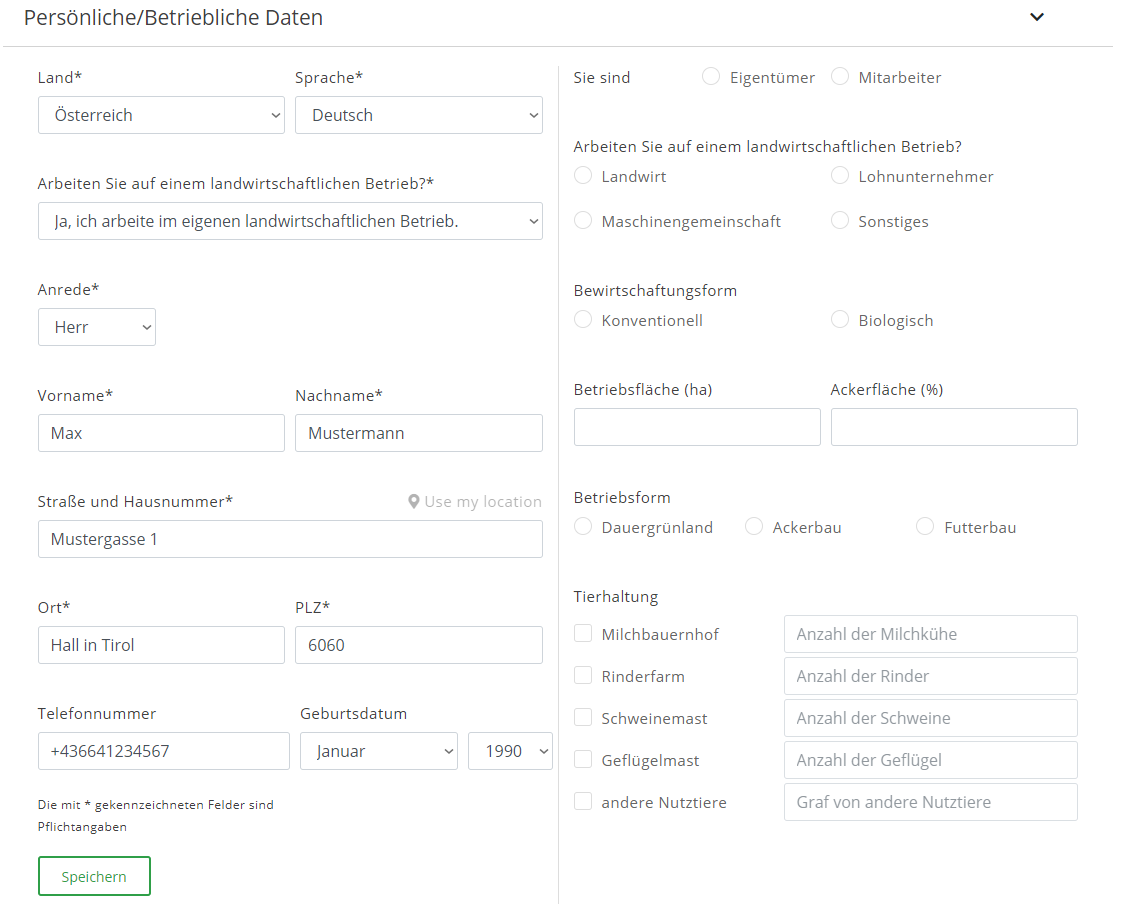
\includegraphics[width=1\textwidth, frame]{./grafiken/erm_profil_daten.png}
	}
	\vskip0pt
	\caption{Persönliche/Betriebliche Daten} \label{fig:profilData}
\end{figure}

Bei den Daten über den Betrieb wird gefragt, wie der Benutzer auf den Betrieb angestellt ist. Weiters ist auszufüllen, um welche Art von landwirtschaftlichen Betrieb es sich handelt. Die Betriebsfläche ist in Hektar und die Ackerfläche in Prozent anzugeben und für die Bewirtschaftungsform stehen Konventionell und Biologisch zur Auswahl. Danach wählt man noch die Betriebsform und die Anzahl der jeweiligen Tiere.

\subsection{Newsletter}

Die Firma Pöttinger bietet Newsletter in verschiedenen Sprachen für die Kunden an. Es besteht die Möglichkeit sich von diesen Newsletter jederzeit an- oder abzumelden. Das geschieht mit einem Klick auf den jeweiligen Knopf unter der gewünschten Sprache. Falls ein Newsletter abonniert ist, sieht man darunter, seit wann man diesen Newsletter erhält.

\begin{figure}[H]
	\centerline{
		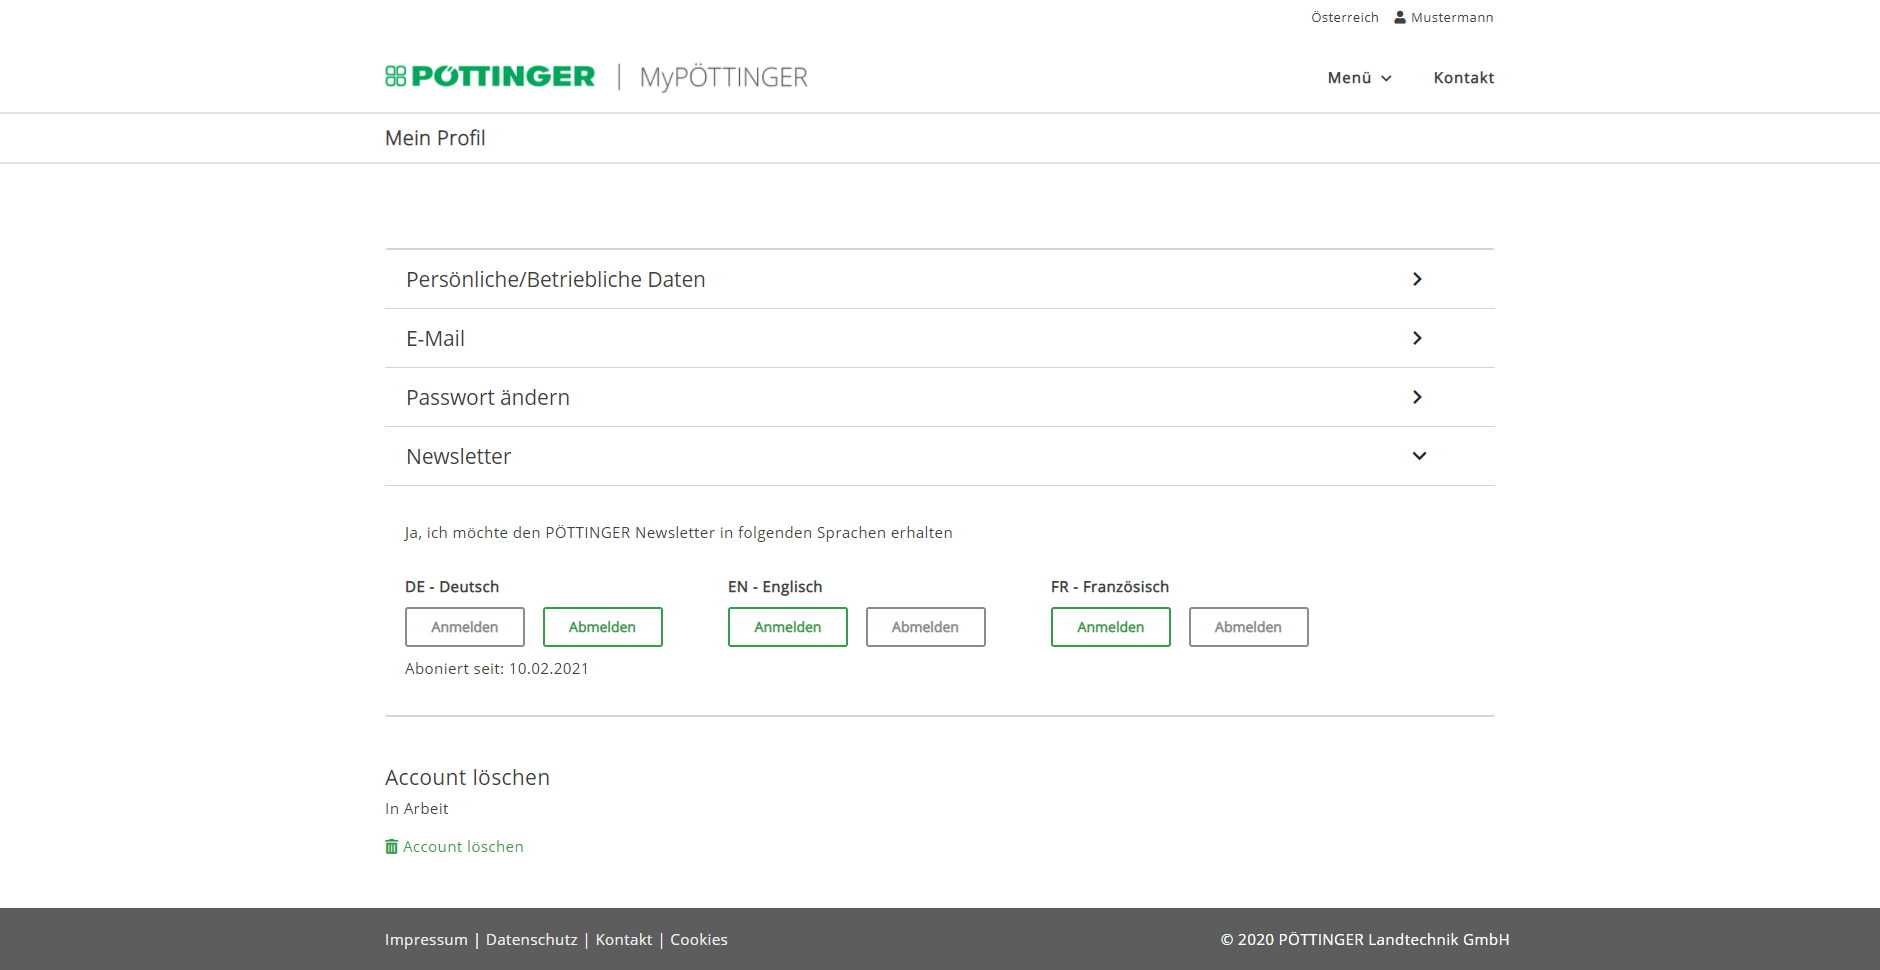
\includegraphics[width=1\textwidth, frame]{./grafiken/erm_profil_newsletter.png}
	}
	\vskip0pt
	\caption{Newsletter} \label{fig:newsletter}
\end{figure}

\section{Produktpalette}

Mit der Produktpalette erhält man eine Vielzahl an Informationen zu den Landmaschinen der Firma Pöttinger. Um die gewünschte Maschine zu finden, gibt es verschiedene Möglichkeiten. Eine Möglichkeit ist, die Maschine in der Produktpalette zu suchen. Dafür klickt man auf "Suche in der Produktpalette" und danach öffnet sich ein Baumstruktur, in der man von oben nach unten in den Kategorien suchen kann. Am Beginn stehen Grünland und Ackerbau zur Auswahl. Öffnet man Grünland, erscheinen die Unterkategorien dieser Kategorie. Es gibt bis zu fünf Ebenen, bis man zu den einzelnen Maschinen gelangt. Diese Suche in der Baumstruktur kann man mit einer Eingabe in der Stichwortsuche über dem Baum noch einschränken. Wenn das eingegebene Stichwort in einer Ebene und darunter nicht vorkommt, sieht man diese Ebene auch nicht mehr. In Abbildung \ref{fig:produktpalette} sieht man die geschlossene Produktpalette. In der Abbildung \ref{fig:produktpaletteOffen} sieht man ein Beispiel für Produktpalette mit offenen Unterebenen und in Abbildung \ref{fig:produktpaletteMitStichwort} sieht man den Unterschied, wenn man die offene Produktpalette mit einer Stichworteingabe verbindet.

\begin{figure}[H]
	\centerline{
		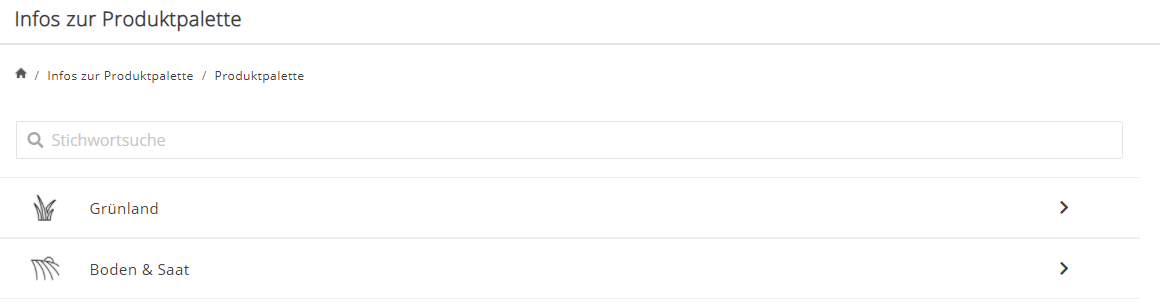
\includegraphics[width=1\textwidth, frame]{./grafiken/erm_produktpalette_neu_.png}
	}
	\vskip0pt
	\caption{Produktpalette} \label{fig:produktpalette}
\end{figure}

\begin{figure}[H]
	\centerline{
		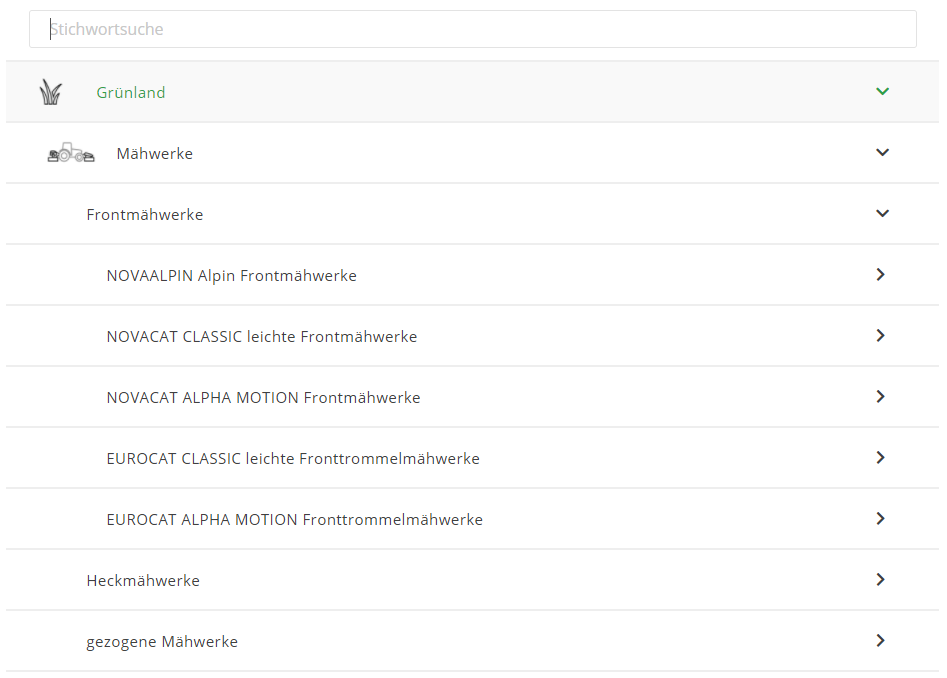
\includegraphics[width=1\textwidth, frame]{./grafiken/erm_produktpalette_offen.png}
	}
	\vskip0pt
	\caption{Offene Produktpalette} \label{fig:produktpaletteOffen}
\end{figure}

\begin{figure}[H]
	\centerline{
		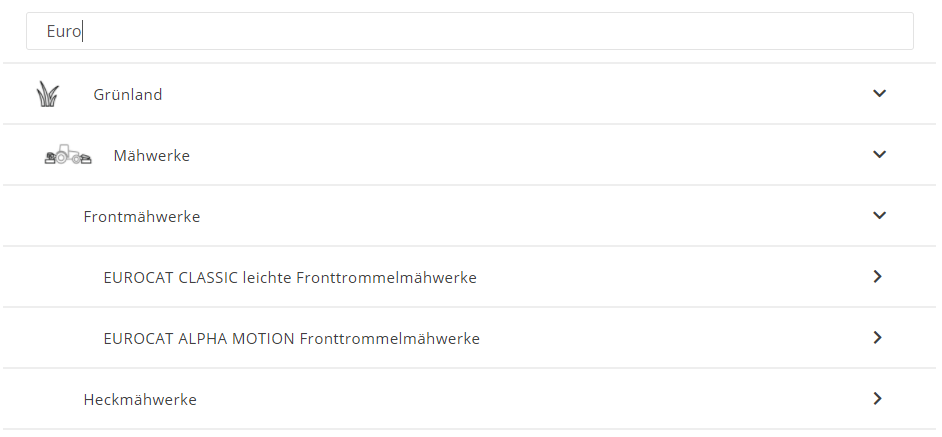
\includegraphics[width=1\textwidth, frame]{./grafiken/erm_produktpalette_offen_stichwort.PNG}
	}
	\vskip0pt
	\caption{Offene Produktpalette mit Stichwortsuche} \label{fig:produktpaletteMitStichwort}
\end{figure}

Eine andere Möglichkeit ist noch die Suche mit einer gültigen Maschinennummer. Gibt man diese Nummer ein, gelangt man direkt zur Produktübersicht.

\section{Produktübersicht}

Hat man sich eine Maschine in der Produktpalette, direkt mit der Maschinennummer oder eine in Maschinenpark gespeicherte Maschine gesucht, gelangt man auf die Produktübersicht, die man in Abbildung \ref{fig:produktübersicht} sehen kann. Hier findet man jegliche nützliche Information der ausgewählten Maschine. Die angezeigten Informationen variieren je nach Maschine und Verfügbarkeit.

\begin{figure}[H]
	\centerline{
		\includegraphics[width=1\textwidth, frame]{./grafiken/erm_produktübersicht.png}
	}
	\vskip0pt
	\caption{Produktübersicht} \label{fig:produktübersicht}
\end{figure}

\subsection{Highlights}

Bei den Highlights des Produktes werden wissenswerte Informationen in Form eines Bildes mit einer Überschrift aufgelistet. Das sieht man in Abbildung \ref{fig:highlight}.
\begin{figure}[H]
	\centerline{
		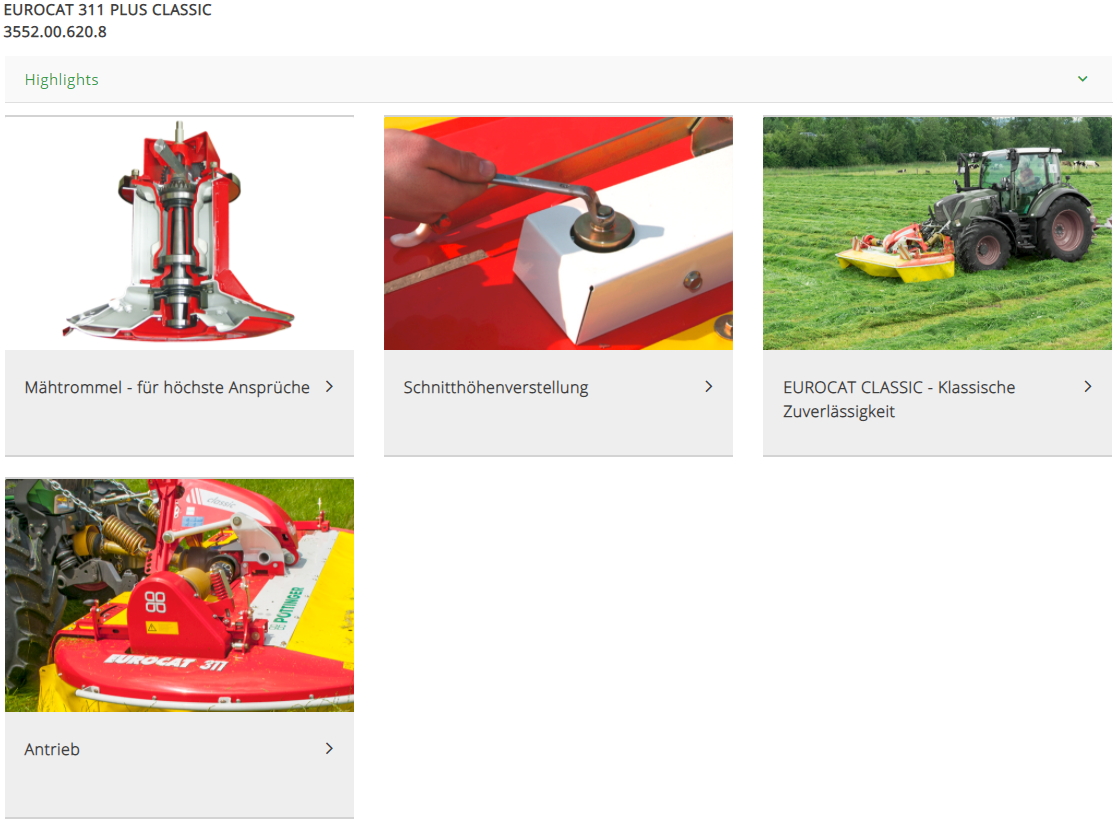
\includegraphics[width=1\textwidth, frame]{./grafiken/erm_detailansicht_highlights.PNG}
	}
	\vskip0pt
	\caption{Highlights} \label{fig:highlight}
\end{figure}
 Wird nun ein Highlight ausgewählt, gelangt man zu einer genaueren Beschreibung der jeweiligen Besonderheit. So einen Artikel sieht man in Abbildung \ref{fig:highlightbeschreibung}.
\begin{figure}[H]
	\centerline{
		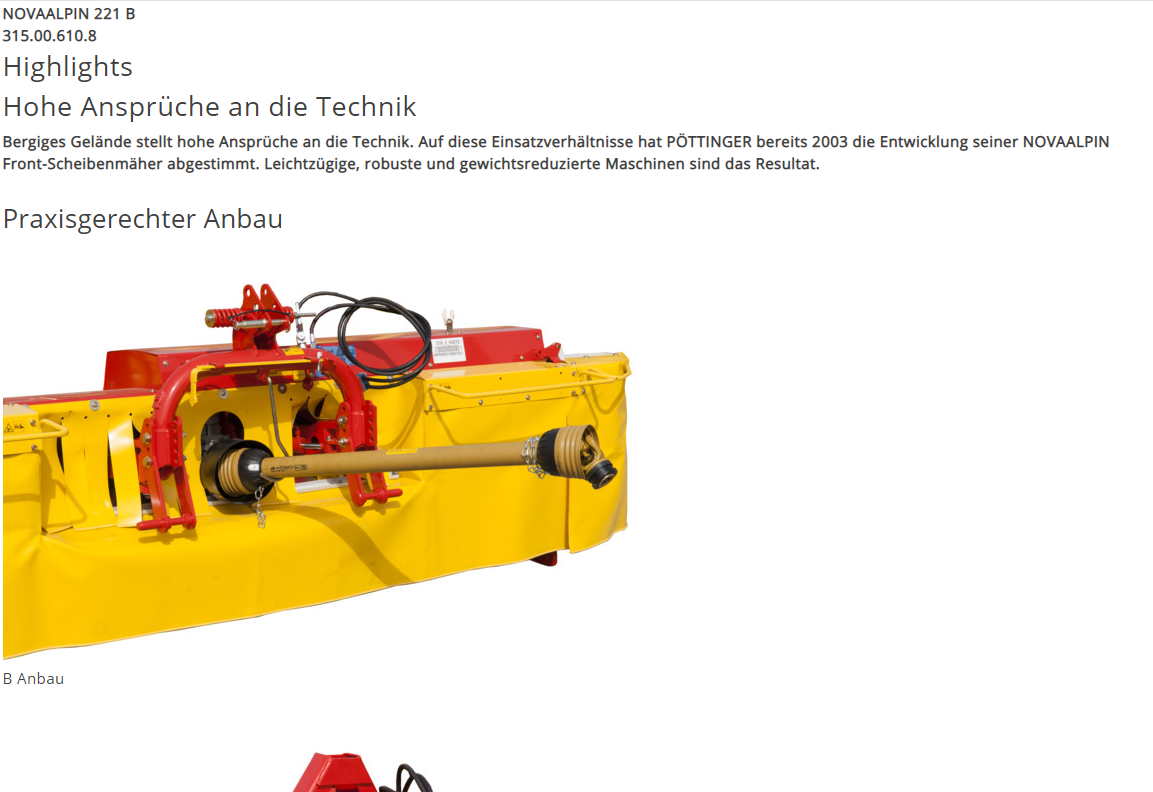
\includegraphics[width=1\textwidth, frame]{./grafiken/erm_detailansicht_highlights_beschreibung.PNG}
	}
	\vskip0pt
	\caption{Highlight-Beschreibung} \label{fig:highlightbeschreibung}
\end{figure}

\subsection{Ausstattung}

Bei der Ausstattung findet man die verbauten Teile. Wie in Abbildung \ref{fig:ausstattung} sieht man diese Teile mit der jeweiligen Materialnummer und einer Bezeichnung aufgelistet. Darunter sieht man noch optionale Ausrüstungen, die mit dieser Maschine kompatibel sind.

\begin{figure}[H]
	\centerline{
		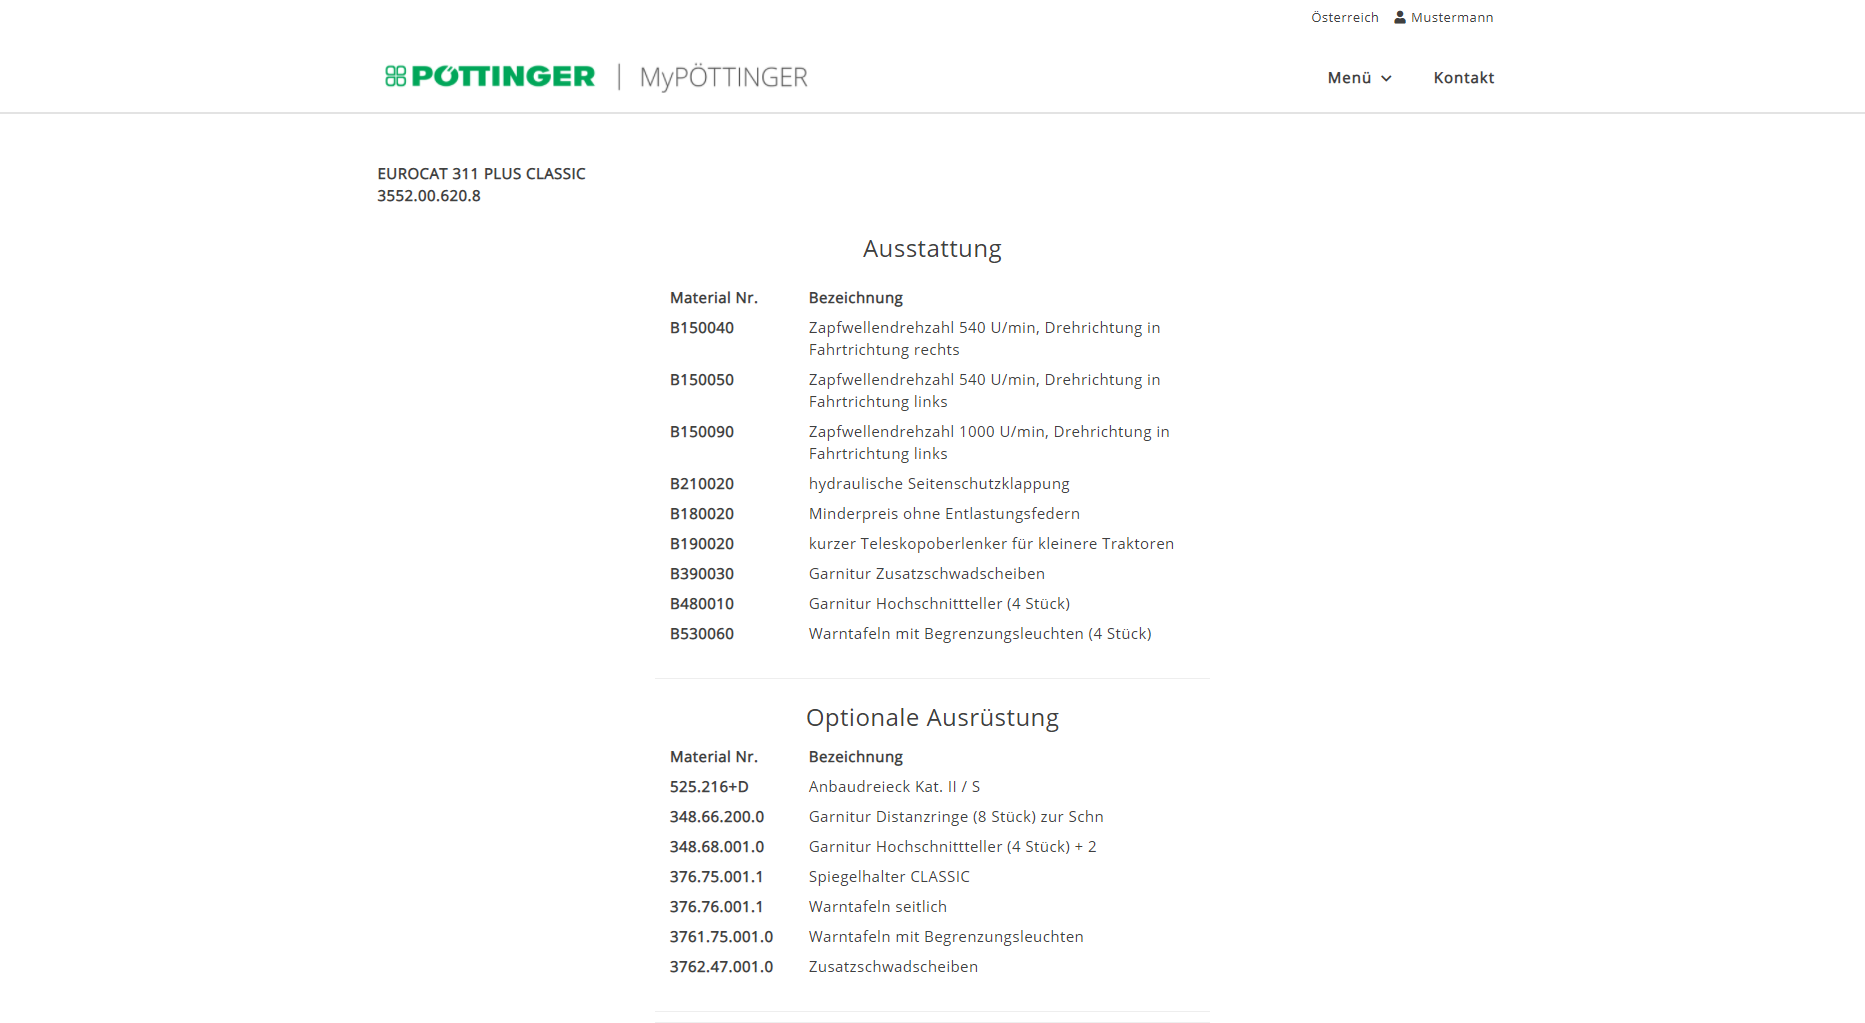
\includegraphics[width=1\textwidth, frame]{./grafiken/erm_detailansicht_ausstattung.PNG}
	}
	\vskip0pt
	\caption{Ausstattung} \label{fig:ausstattung}
\end{figure}

\subsection{Technische Daten}

Bei den technischen Daten in Abbildung \ref{fig:technischeDaten} findet man nützliche Informationen wie Anbau, Gewicht, Arbeitsbreite, Transportbreite, Kraftbedarf und vieles mehr.

\begin{figure}[H]
	\centerline{
		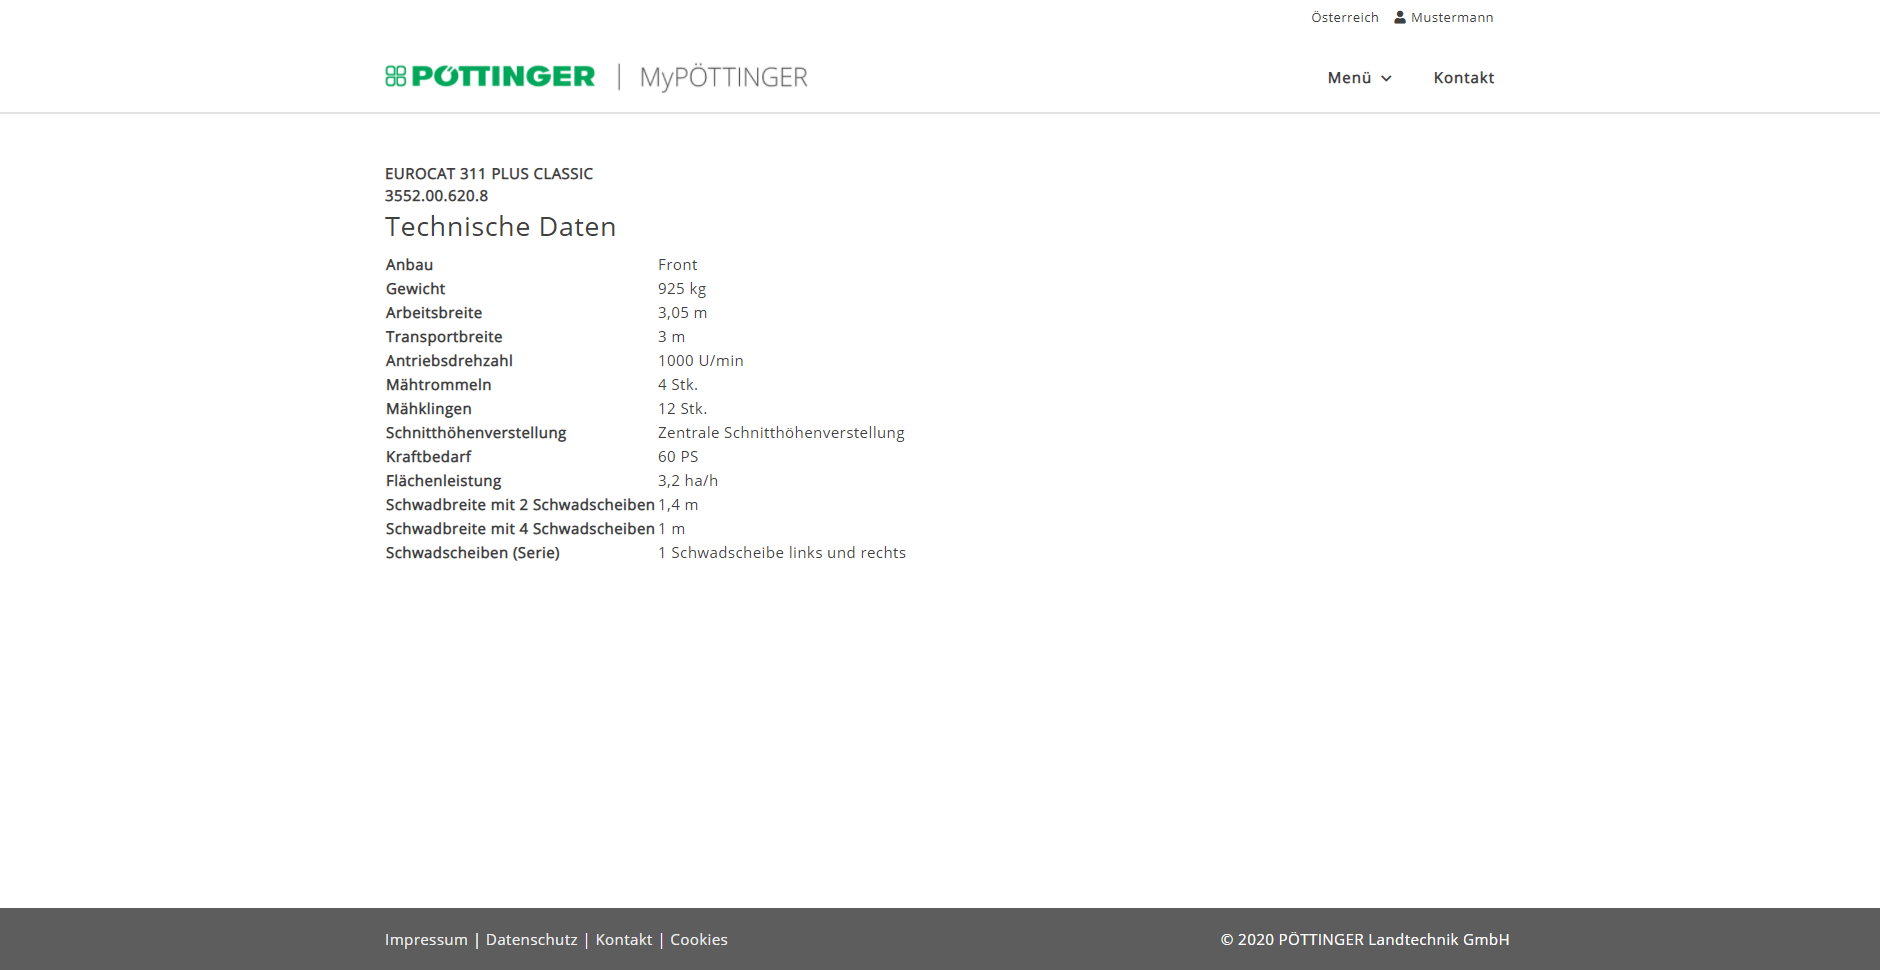
\includegraphics[width=1\textwidth, frame]{./grafiken/erm_detailansicht_technisch.PNG}
	}
	\vskip0pt
	\caption{Ausstattung} \label{fig:technischeDaten}
\end{figure}
\subsection{Videos, Bilder, Prospekte und Betriebsanleitung}
In diesen Kategorien findet man Videos, Bilder, Prospekte und eine Betriebsanleitung für die Maschine. Diese Videos werden über YouTube abgespielt. Die Prospekte und die Betriebsanleitung sind zum Download verfügbar. Da nicht von jeder Maschine Bilder oder Videos vorhanden sind, Gibt es dieses Feld auch nicht bei jeder Detailansicht.
\section{Maschinenpark}

In Abbildung \ref{fig:maschinenpark} sieht man den Maschinenpark, in dem eine Auflistung aller gespeicherten Maschinen des Benutzers ist. Somit hat der Nutzer einen schnellen Zugriff auf nützliche Tipps zur der gespeicherten Maschine, Bedienungsanleitungen, Ersatzteillisten, Wartungsinformationen, sowie alle technischen Details und Unterlagen.

\begin{figure}[H]
	\centerline{
		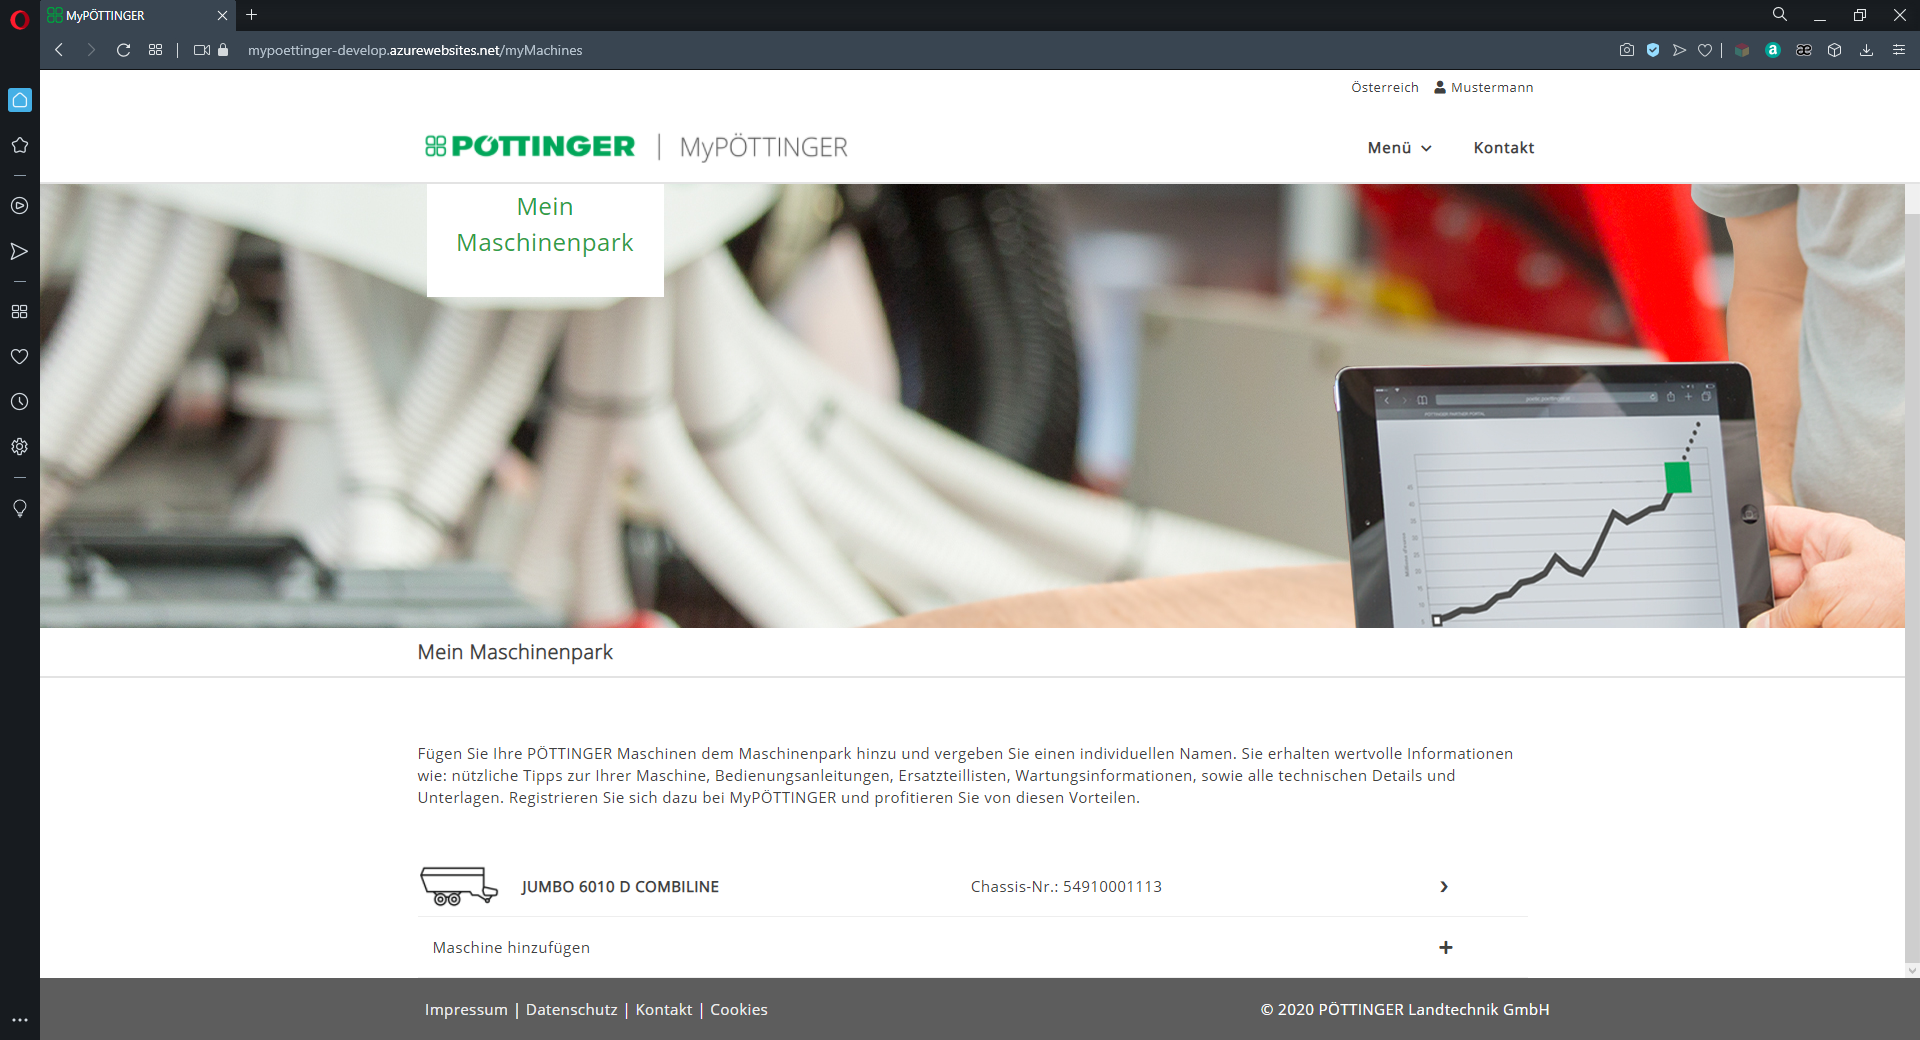
\includegraphics[width=1\textwidth, frame]{./grafiken/erm_maschinenpark.png}
	}
	\vskip0pt
	\caption{Maschinenpark} \label{fig:maschinenpark}
\end{figure}

Navigiert man über den Maschinenpark zu der gespeicherten Maschine, ändert sich die Detailansicht, wie in Abbildung \ref{fig:savedMaschine}, etwas. Hinzugekommen ist ein Bild der Maschine und es bietet die Möglichkeit, diese Maschine einen individuellen Namen zu vergeben.

\begin{figure}[H]
	\centerline{
		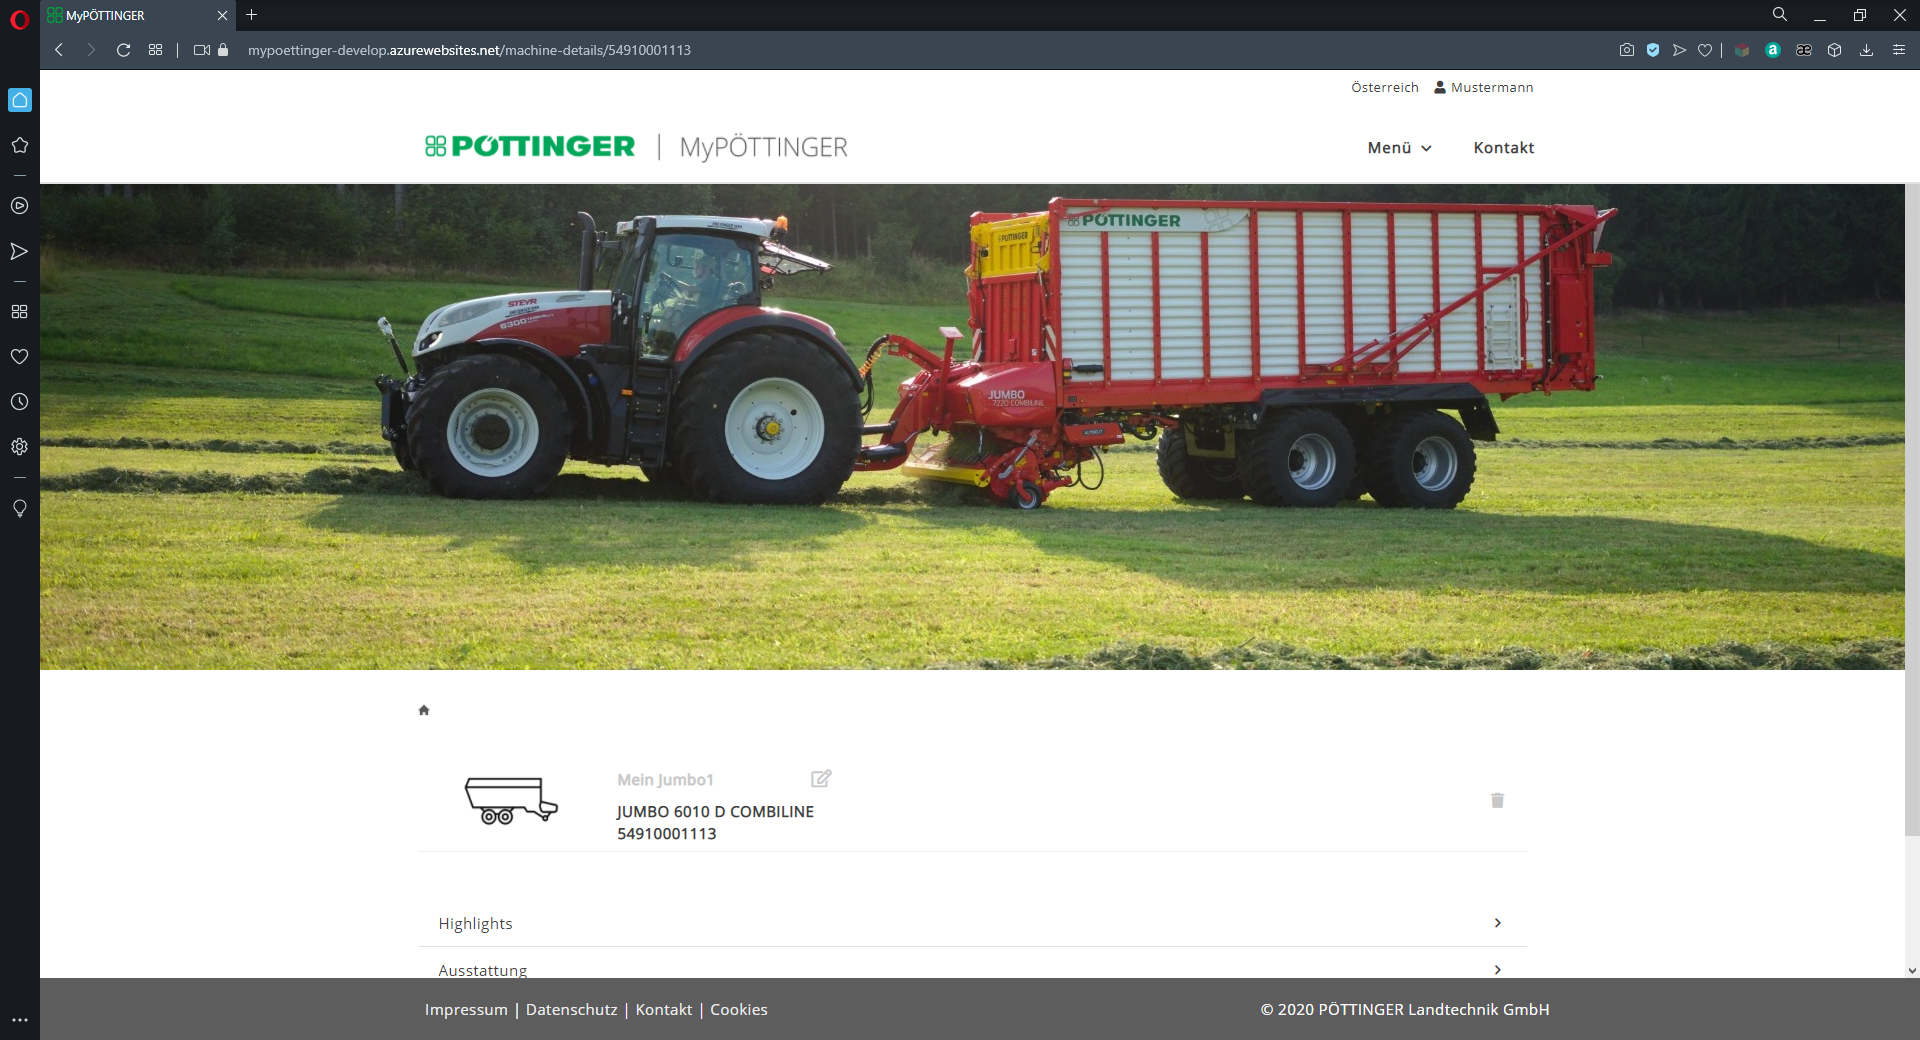
\includegraphics[width=1\textwidth, frame]{./grafiken/erm_detailansicht_saved_machine.png}
	}
	\vskip0pt
	\caption{Detailansicht der gespeicherten Maschine} \label{fig:savedMaschine}
\end{figure}

Wenn die Maschine einen individuellen Namen erhalten hat, wird dieser Name auch im eigenen Maschinenpark wie in Abbildung \ref{fig:benannteMaschine} angezeigt:
 
\begin{figure}[H]
	\centerline{
		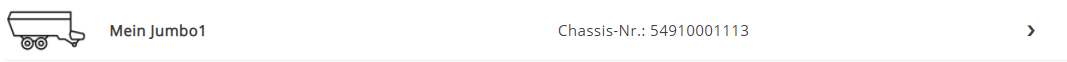
\includegraphics[width=1\textwidth, frame]{./grafiken/erm_maschinenpark_benannteMaschine.png}
	}
	\vskip0pt
	\caption{Benannte Maschine} \label{fig:benannteMaschine}
\end{figure}